\documentclass[a4paper,twocolumn,11pt,nopdfoutputerror]{quantumarticle}
%DIF LATEXDIFF DIFFERENCE FILE
%DIF DEL STAR_GNN_BB_v2.tex   Sun Sep 27 18:52:35 2026
%DIF ADD STAR_GNN_BB_v3.tex   Sun Sep 27 19:43:07 2026
\usepackage[utf8]{inputenc}
\usepackage[T1]{fontenc}
\usepackage[english]{babel}
\usepackage{amsmath,amssymb,amsthm,mathtools}
\usepackage{braket}
\usepackage{graphicx}
\usepackage{booktabs}
\usepackage{siunitx}
\usepackage{microtype}
\usepackage{xcolor}
\usepackage[numbers,sort&compress]{natbib}
\usepackage[ruled,vlined]{algorithm2e}
\usepackage{enumitem}
\usepackage{multirow}
\usepackage{bbm}
\usepackage{makecell}

% ---------- macros ----------
\DeclareMathOperator{\Tr}{Tr}
\newcommand{\F}{\mathbb{F}}
\newcommand{\R}{\mathbb{R}}
\newcommand{\Pauli}{\mathcal{P}}
\newcommand{\synd}{\mathbf{s}}
\newcommand{\err}{\mathbf{e}}
\newcommand{\ehat}{\hat{\mathbf{e}}}
\newcommand{\llr}{\Lambda}
\newcommand{\Hmat}{\mathbf{H}}
\newcommand{\Gmat}{\mathbf{G}}
\newcommand{\Wmat}{\mathbf{W}}
\newcommand{\bvec}[1]{\mathbf{#1}}
\newcommand{\phat}{\hat{p}}
\newcommand{\concat}{\,\|\,}
\newcommand{\code}[3]{\ensuremath{[\![#1,#2,#3]\!]}}
\newcommand{\pending}[1]{\textcolor{red}{\textbf{[#1]}}}
\newtheorem{proposition}{Proposition}
\newtheorem{remark}{Remark}

\graphicspath{{./figures/}{./}}
\DeclareGraphicsExtensions{.pdf,.png,.jpg}

\usepackage{hyperref}
\hypersetup{colorlinks=true,citecolor=blue,linkcolor=blue,urlcolor=blue}

% ============================================================
%  TITLE
% ============================================================
%DIF 48c48
%DIF < \title{GNN-Augmented Belief Propagation for Bivariate Bicycle Codes: Gains, Baseline Sensitivity, and Calibration Side Information}
%DIF -------
\title{GNN-Augmented BP Architectures for QLDPC Decoding} %DIF > 
%DIF -------

\author{Jothiradithya Sai Konduru}
\affiliation{Paradise Valley High School, Phoenix, AZ, USA}

\author{Anish Chedalla}
\affiliation{Paradise Valley High School, Phoenix, AZ, USA}

\author{Nithin Raveendran}
\affiliation{Department of Electrical and Computer Engineering,
             University of Arizona, Tucson, AZ, USA}
\email{nithin@arizona.edu}
%DIF PREAMBLE EXTENSION ADDED BY LATEXDIFF
%DIF UNDERLINE PREAMBLE %DIF PREAMBLE
\RequirePackage[normalem]{ulem} %DIF PREAMBLE
\RequirePackage{color}\definecolor{RED}{rgb}{1,0,0}\definecolor{BLUE}{rgb}{0,0,1} %DIF PREAMBLE
\providecommand{\DIFaddtex}[1]{{\protect\color{blue}\uwave{#1}}} %DIF PREAMBLE
\providecommand{\DIFdeltex}[1]{{\protect\color{red}\sout{#1}}}                      %DIF PREAMBLE
%DIF SAFE PREAMBLE %DIF PREAMBLE
\providecommand{\DIFaddbegin}{} %DIF PREAMBLE
\providecommand{\DIFaddend}{} %DIF PREAMBLE
\providecommand{\DIFdelbegin}{} %DIF PREAMBLE
\providecommand{\DIFdelend}{} %DIF PREAMBLE
\providecommand{\DIFmodbegin}{} %DIF PREAMBLE
\providecommand{\DIFmodend}{} %DIF PREAMBLE
%DIF FLOATSAFE PREAMBLE %DIF PREAMBLE
\providecommand{\DIFaddFL}[1]{\DIFadd{#1}} %DIF PREAMBLE
\providecommand{\DIFdelFL}[1]{\DIFdel{#1}} %DIF PREAMBLE
\providecommand{\DIFaddbeginFL}{} %DIF PREAMBLE
\providecommand{\DIFaddendFL}{} %DIF PREAMBLE
\providecommand{\DIFdelbeginFL}{} %DIF PREAMBLE
\providecommand{\DIFdelendFL}{} %DIF PREAMBLE
%DIF HYPERREF PREAMBLE %DIF PREAMBLE
\providecommand{\DIFadd}[1]{\texorpdfstring{\DIFaddtex{#1}}{#1}} %DIF PREAMBLE
\providecommand{\DIFdel}[1]{\texorpdfstring{\DIFdeltex{#1}}{}} %DIF PREAMBLE
%DIF COLORLISTINGS PREAMBLE %DIF PREAMBLE
\RequirePackage{listings} %DIF PREAMBLE
\RequirePackage{color} %DIF PREAMBLE
\lstdefinelanguage{DIFcode}{ %DIF PREAMBLE
%DIF DIFCODE_UNDERLINE %DIF PREAMBLE
  moredelim=[il][\color{red}\sout]{\%DIF\ <\ }, %DIF PREAMBLE
  moredelim=[il][\color{blue}\uwave]{\%DIF\ >\ } %DIF PREAMBLE
} %DIF PREAMBLE
\lstdefinestyle{DIFverbatimstyle}{ %DIF PREAMBLE
	language=DIFcode, %DIF PREAMBLE
	basicstyle=\ttfamily, %DIF PREAMBLE
	columns=fullflexible, %DIF PREAMBLE
	keepspaces=true %DIF PREAMBLE
} %DIF PREAMBLE
\lstnewenvironment{DIFverbatim}{\lstset{style=DIFverbatimstyle}}{} %DIF PREAMBLE
\lstnewenvironment{DIFverbatim*}{\lstset{style=DIFverbatimstyle,showspaces=true}}{} %DIF PREAMBLE
%DIF END PREAMBLE EXTENSION ADDED BY LATEXDIFF

\begin{document}
\maketitle

% ============================================================
%  ABSTRACT
% ============================================================
\begin{abstract}
Bivariate bicycle (BB) quantum low-density parity-check (QLDPC) codes
combine finite encoding rate with low-weight checks, but their loopy
Tanner graphs remain challenging for iterative decoding. \DIFdelbegin \DIFdel{Learned
message-passing can improve belief propagation (BP), although the
measured gain depends strongly on the BP configuration used for
training and evaluation. We study this issue using }\DIFdelend \DIFaddbegin \DIFadd{We study }\DIFaddend a
Tanner-graph neural network (\textsc{TannerGNN}) that produces
qubit-wise log-likelihood corrections for \DIFdelbegin \DIFdel{BP under a biased CSS component-noise model}\DIFdelend \DIFaddbegin \DIFadd{belief propagation (BP) under
$Z$-biased noise ($\eta=20$), and ask how its gain depends on the decoder
it is compared against}\DIFaddend . On the $\code{72}{12}{6}$ BB code, a model trained
\DIFdelbegin \DIFdel{with }\DIFdelend \DIFaddbegin \DIFadd{through }\DIFaddend 10-iteration flooding BP reduces the logical error rate (LER) \DIFdelbegin \DIFdel{from $0.0990$ to $0.0838$ on
8}\DIFdelend \DIFaddbegin \DIFadd{of
that decoder by $12.5\%\pm0.6\%$ at $p=0.04$ and by $10.6\%\pm0.7\%$ at
$p=0.06$, outside the training range (five training seeds, 20}\DIFaddend {,}000 \DIFaddbegin \DIFadd{and
10}{\DIFadd{,}}\DIFadd{000 }\DIFaddend held-out \DIFdelbegin \DIFdel{syndromes at $p=0.04$ and
$\eta=20$,a $15.4\%$
relative reduction (paired McNemar $p<10^{-15}$). This gain does not
transfer to a stronger serial min-sum }\DIFdelend \DIFaddbegin \DIFadd{shots, every seed McNemar $p<10^{-36}$). The gain comes
mainly from helping BP converge, and it does not reach longer decoding:
100-iteration BP and serial }\DIFaddend BP-OSD \DIFdelbegin \DIFdel{decoder: the learned
correction is statistically indistinguishable at lower tested error
rates and degrades performance at $p\geq 0.04$. Independent baseline
experiments further show that schedule, BP update rule, iteration count,
and OSD
configuration can }\DIFdelend \DIFaddbegin \DIFadd{both outperform GNN-augmented
10-iteration BP, and the same corrections make BP-OSD slightly worse. A
paired failure-set analysis shows why: the failure sets of BP and BP-OSD
are nested, and most shots the GNN repairs are shots BP-OSD already
decodes. Baseline experiments show that BP schedule and OSD
post-processing }\DIFaddend change LER by \DIFdelbegin \DIFdel{orders of magnitude. These
settings must therefore be specified and controlled when }\DIFdelend \DIFaddbegin \DIFadd{about $47\times$ on
$\code{288}{12}{18}$, so these settings must be specified whenever
}\DIFaddend learned decoders are compared. We \DIFdelbegin \DIFdel{also establish that }\DIFdelend \DIFaddbegin \DIFadd{prove that the hard decisions of
}\DIFaddend unclipped min-sum BP \DIFdelbegin \DIFdel{is invariant , in its hard
decisions, }\DIFdelend \DIFaddbegin \DIFadd{are invariant }\DIFaddend to a uniform \DIFdelbegin \DIFdel{positive rescaling of all channel
LLRswithin a
CSS component. Thus, changing only the magnitude of a uniform prior
cannot make the underlying }\DIFdelend \DIFaddbegin \DIFadd{rescaling of the channel
LLRs, so a global noise estimate alone cannot make }\DIFaddend min-sum BP adaptive\DIFdelbegin \DIFdel{, although a learned
network may still use global context through other pathways.
Finally, synthetic experiments with heterogeneous }\DIFdelend \DIFaddbegin \DIFadd{.
In contrast, revealing true }\DIFaddend per-qubit error rates \DIFdelbegin \DIFdel{show a
large gap between mean-prior and oracle-prior decoding, motivating
}\DIFdelend \DIFaddbegin \DIFadd{reduces BP-OSD's LER by
$65$--$88\%$ under heterogeneous code-capacity noise ($\sigma=1$) and by
$56\%$ under circuit-level noise, identifying }\DIFaddend spatially resolved
calibration \DIFdelbegin \DIFdel{side information rather than a single
global noise scalar. The experiments show that an improvement over one BP baseline does not
by itself establish an improvement over a stronger decoder, and that
spatial calibration information is qualitatively different from a single
global noise estimate}\DIFdelend \DIFaddbegin \DIFadd{as the more informative side information}\DIFaddend .
\end{abstract}

% ============================================================
%  I. INTRODUCTION
% ============================================================
\section{Introduction}

Bivariate bicycle (BB) codes provide a concrete finite-length setting in
which QLDPC codes combine non-vanishing encoding rate, weight-six
stabilizer checks, and syndrome-extraction circuits compatible with
low-degree connectivity~\cite{Bravyi2024Memory}. IBM's current
fault-tolerant architecture is explicitly based on BB codes, making the
finite-length decoding behavior of this family practically relevant as
well as theoretically interesting~\cite{IBMRoadmap2025}. The canonical
examples include the $\code{72}{12}{6}$, $\code{144}{12}{12}$, and
$\code{288}{12}{18}$ codes studied here.

The decoding bottleneck is not the absence of efficient iterative
algorithms, but their finite-length failure modes. BP is attractive
because its message updates are local and parallelizable, yet short
cycles and degeneracy in QLDPC Tanner graphs create correlated messages
and non-convergent or incorrect fixed points~\cite{Roffe2020Landscape}.
OSD post-processing can recover many BP failures, while recent learned
decoders use graph neural networks (GNNs) either to replace BP or to
intervene between BP stages~\cite{Gong2024GNN,Maan2025MLBP}. These
approaches make the choice of baseline unusually consequential: a neural
correction trained against one BP schedule or stopping rule need not
address the residual failures of a stronger decoder.

A second issue is adaptivity. Hardware noise is neither spatially nor
temporally uniform, and calibration information can therefore be useful
to a decoder. However, three distinct sources of information should not
be conflated: a global estimate of the physical error rate, spatially
resolved per-qubit calibration data, and syndrome history. A decoder may
respond differently to each. In particular, changing the magnitude of a
uniform channel prior has a restricted effect on min-sum BP, whereas
per-qubit priors can change the relative reliability ordering that drives
both BP and OSD.

We study a GNN-augmented BP pipeline with two questions in view:
\emph{what gain does the learned correction provide relative to the BP
decoder used in training, and what additional information is needed for
noise adaptation?} We compare decoder configurations, training and
evaluation baselines, and different forms of calibration information to
isolate the source of the observed performance changes.

\subsection{Contributions}\label{sec:contributions}

Our main findings are:
\begin{enumerate}[leftmargin=*,topsep=3pt,itemsep=3pt]
\item \textbf{A \DIFdelbegin \DIFdel{held-out }\DIFdelend \DIFaddbegin \DIFadd{reproducible }\DIFaddend GNN gain over \DIFaddbegin \DIFadd{the training decoder, and }\DIFaddend its
\DIFdelbegin \DIFdel{training-aligned BP baseline}\DIFdelend \DIFaddbegin \DIFadd{limits}\DIFaddend .} On $\code{72}{12}{6}$\DIFdelbegin \DIFdel{at $p=0.04$ and $\eta=20$}\DIFdelend , \textsc{TannerGNN} + \DIFaddbegin \DIFadd{10-iteration }\DIFaddend flooding
BP reduces LER \DIFdelbegin \DIFdel{from $0.0990$ to $0.0838$
on 8}%DIFDELCMD < {%%%
\DIFdel{,}%DIFDELCMD < }%%%
\DIFdel{000 held-out syndromes, corresponding to a $15.4\%$ relative
reduction (McNemar $p<10^{-15}$). The model is trained only on
$p\in[0.02,0.03]$, so this test is also outside the training error-rate
range }\DIFdelend \DIFaddbegin \DIFadd{by $12.5\%\pm0.6\%$ at $p=0.04$ and $10.6\%\pm0.7\%$ at
$p=0.06$ over five training seeds, with train, validation and test data
drawn from independent seeds and checkpoints selected on validation data
}\DIFaddend (Sec.~\ref{sec:gnn_positive}). \DIFaddbegin \DIFadd{The corrected decoder remains weaker than
100-iteration BP and serial BP-OSD.
}\DIFaddend 

\item \DIFdelbegin \textbf{\DIFdel{Baseline configuration and alignment can dominate the
apparent learned gain.}} %DIFAUXCMD
\DIFdel{Serial min-sum BP with OSD post-processing is
substantially stronger than
the flooding BP used in GNN training.
}\DIFdelend \DIFaddbegin \textbf{\DIFadd{The training decoder and the evaluation decoder are part of
the experimental condition.}} \DIFadd{The same corrections do not improve serial
BP-OSD and are significantly worse in 14 of 15 seed--error-rate pairs
from $p=0.03$ on. }\DIFaddend The \DIFdelbegin \DIFdel{same learned correction does not improve this stronger decoder and is
worse at the two highest tested error rates. Separate experiments on}\DIFdelend \DIFaddbegin \DIFadd{failure sets of BP
and BP-OSD are nested (93\% of BP-OSD failures are BP failures), and
64--69\% of the shots the GNN repairs are already decoded correctly by
BP-OSD. On }\DIFaddend $\code{288}{12}{18}$\DIFdelbegin \DIFdel{show order-of-magnitude sensitivity to BP schedule,
update rule, iteration count, and OSD settings. The training decoder and evaluation decoder are therefore part of the
experimental condition rather than interchangeable implementations of ``BP ''
}\DIFdelend \DIFaddbegin \DIFadd{, changing only the BP schedule and then
adding OSD-CS-10 lowers LER by $8.8\times$ and $5.4\times$
}\DIFaddend (Secs.~\ref{sec:baseline} and~\ref{sec:mismatch}).

\item \textbf{Global prior scaling and spatial calibration carry
different information.} \DIFdelbegin \DIFdel{We prove that hard }\DIFdelend \DIFaddbegin \DIFadd{Hard }\DIFaddend decisions of unclipped min-sum BP are
invariant to a uniform positive rescaling of the channel LLRs within a
CSS component. \DIFdelbegin \DIFdel{This result limits adaptivity obtained only
by changing a uniform BP prior; it does not rule out a learned network
using a global noise scalar as context. In synthetic heterogeneous-noise
experiments, providing the }\DIFdelend \DIFaddbegin \DIFadd{In contrast, providing }\DIFaddend true per-qubit rates to BP-OSD
\DIFdelbegin \DIFdel{yields large
oracle improvements, motivating spatially resolved calibration inputs.
Because code size and operating point co-vary in these experiments, we do
not attribute the cross-code trend to distance alone
}\DIFdelend \DIFaddbegin \DIFadd{reduces LER by up to $88\%$ at code capacity and by $56\%$ at circuit
level }\DIFaddend (Secs.~\ref{sec:invariance}\DIFdelbegin \DIFdel{and~\ref{sec:oraclegap}}\DIFdelend \DIFaddbegin \DIFadd{, \ref{sec:oraclegap}
and~\ref{sec:circuit}}\DIFaddend ).
\end{enumerate}
\section{Background}\label{sec:background}

\subsection{CSS codes and bivariate bicycle construction}

A CSS code~\cite{Calderbank1996Good,Steane1996Error} is defined by
matrices $\Hmat_x, \Hmat_z \in \F_2^{m \times n}$ with
$\Hmat_x \Hmat_z^\top = \mathbf{0}$. The syndrome of an error
$(e_x, e_z)$ decomposes as
$s_x = \Hmat_x e_z$,
$s_z = \Hmat_z e_x$
over $\F_2$, so $X$- and $Z$-type errors are decoded independently.
This CSS independence is structurally important for the results
of Sec.~\ref{sec:invariance}.

Bivariate bicycle codes~\cite{Bravyi2024Memory} are constructed
over the group algebra $\F_2[x,y]/(x^\ell-1,\,y^m-1)$. Polynomials
$A(x,y)$ and $B(x,y)$ yield circulant block matrices:
\begin{equation}
\Hmat_x = [\mathbf{A} \mid \mathbf{B}], \qquad
\Hmat_z = [\mathbf{B}^\top \mid \mathbf{A}^\top].
\label{eq:bb}
\end{equation}
We study three codes (Table~\ref{tab:codes}).

\begin{table}[t]
\centering
\small
\caption{Bivariate bicycle codes studied in this work\DIFdelbeginFL \DIFdelFL{, with
         generator polynomials from }\DIFdelendFL \DIFaddbeginFL \DIFaddFL{~}\DIFaddendFL \cite{Bravyi2024Memory}.
         \DIFaddbeginFL \DIFaddFL{$\Hmat_x=[\mathbf{A}\mid\mathbf{B}]$ and
         $\Hmat_z=[\mathbf{B}^\top\mid\mathbf{A}^\top]$ over
         $\F_2[x,y]/(x^\ell-1,\,y^m-1)$.}\DIFaddendFL }
\label{tab:codes}
\DIFdelbeginFL %DIFDELCMD < \begin{tabular}{@{}lcccccc@{}}
%DIFDELCMD < \toprule
%DIFDELCMD < %%%
\DIFdelFL{Code }%DIFDELCMD < & %%%
\DIFdelFL{$n$ }%DIFDELCMD < & %%%
\DIFdelFL{$k$ }%DIFDELCMD < & %%%
\DIFdelFL{$d$ }%DIFDELCMD < & %%%
\DIFdelFL{Rate }%DIFDELCMD < & %%%
\DIFdelFL{$\ell$ }%DIFDELCMD < & %%%
\DIFdelFL{$m$ }%DIFDELCMD < \\
%DIFDELCMD < \midrule
%DIFDELCMD < %%%
\DIFdelFL{$\code{72}{12}{6}$   }%DIFDELCMD < &  %%%
\DIFdelFL{72 }%DIFDELCMD < & %%%
\DIFdelFL{12 }%DIFDELCMD < &  %%%
\DIFdelFL{6 }%DIFDELCMD < & %%%
\DIFdelFL{1/6  }%DIFDELCMD < &  %%%
\DIFdelFL{6 }%DIFDELCMD < &  %%%
\DIFdelFL{6 }%DIFDELCMD < \\
%DIFDELCMD < %%%
\DIFdelFL{$\code{144}{12}{12}$ }%DIFDELCMD < & %%%
\DIFdelFL{144 }%DIFDELCMD < & %%%
\DIFdelFL{12 }%DIFDELCMD < & %%%
\DIFdelFL{12 }%DIFDELCMD < & %%%
\DIFdelFL{1/12 }%DIFDELCMD < & %%%
\DIFdelFL{12 }%DIFDELCMD < &  %%%
\DIFdelFL{6 }%DIFDELCMD < \\
%DIFDELCMD < %%%
\DIFdelFL{$\code{288}{12}{18}$ }%DIFDELCMD < & %%%
\DIFdelFL{288 }%DIFDELCMD < & %%%
\DIFdelFL{12 }%DIFDELCMD < & %%%
\DIFdelFL{18 }%DIFDELCMD < & %%%
\DIFdelFL{1/24 }%DIFDELCMD < & %%%
\DIFdelFL{12 }%DIFDELCMD < & %%%
\DIFdelFL{12 }%DIFDELCMD < \\
%DIFDELCMD < \bottomrule
%DIFDELCMD < \end{tabular}
%DIFDELCMD < %%%
\DIFdelendFL \DIFaddbeginFL \resizebox{\columnwidth}{!}{%
\begin{tabular}{@{}lccccl@{}}
\toprule
Code & Name & $\ell$ & $m$ & $A(x,y)$ & $B(x,y)$ \\
\midrule
$\code{72}{12}{6}$   & ---        &  6 &  6 & $x^3+y+y^2$   & $y^3+x+x^2$ \\
$\code{144}{12}{12}$ & gross      & 12 &  6 & $x^3+y+y^2$   & $y^3+x+x^2$ \\
$\code{288}{12}{18}$ & two-gross  & 12 & 12 & $x^3+y^2+y^7$ & $y^3+x+x^2$ \\
\bottomrule
\end{tabular}}
\DIFaddendFL \end{table}

\subsection{Belief propagation and its failure modes}\label{sec:bp}

Min-sum BP on a CSS Tanner graph iterates variable-to-check and
check-to-variable messages for $T$ steps. For a check $c_j$ with measured
syndrome bit $s_j$ and a neighboring variable $v_i$,
\begin{align}
\mu_{v_i \to c_j}^{(t)}
&= \llr_i + \!\!\sum_{j' \in \mathcal{N}(i)\setminus j}\!\!
\mu_{c_{j'} \to v_i}^{(t-1)},
\label{eq:vtc}\\
\mu_{c_j \to v_i}^{(t)}
&= (-1)^{s_j}
\!\!\prod_{i' \in \mathcal{N}(j)\setminus i}\!\!
\mathrm{sgn}\!\left(\mu_{v_{i'}\to c_j}^{(t)}\right) \notag\\
&\quad \times
\!\!\min_{i'\in\mathcal{N}(j)\setminus i}\!\!
\left|\mu_{v_{i'}\to c_j}^{(t)}\right|.
\label{eq:ctv}
\end{align}
The channel LLR for qubit $i$ under $Z$-biased noise is
$\llr_{z,i} = \ln\bigl((1-p_z)/p_z\bigr)$,
$p_z = p\eta/(\eta+1)$.
CSS decoding separates $X$ and $Z$ components, processing each with
its respective parity-check matrix.

The Tanner graphs of the finite-length BB codes considered here contain
many short cycles. Message reuse around these cycles creates statistical
dependencies that are absent on a tree and can lead BP to oscillate,
converge to a syndrome-inconsistent estimate, or converge to the wrong
logical class. We therefore treat short-cycle structure as a finite-length
decoder mechanism to be measured, rather than attributing every cycle
directly to the CSS orthogonality condition. Post-processing methods
including ordered-statistics decoding (OSD)~\cite{Fossorier1995OSD}
recover many such failures but add $O(n^3)$ worst-case complexity.
As shown in Sec.~\ref{sec:baseline}, the specific OSD
\emph{configuration}---schedule, base method, and iteration count---can
change LER by more than two orders of magnitude on the same code. We
therefore report these settings explicitly in the comparisons below.

\subsection{Noise models}\label{sec:noise}

\DIFdelbegin \DIFdel{We use }\DIFdelend \DIFaddbegin \paragraph{\DIFadd{Code capacity.}} \DIFadd{Each data qubit independently suffers a $Z$
flip with probability $p_z$ and an $X$ flip with probability $p_x$,
}\begin{equation}
\DIFadd{p_z = \frac{p\eta}{\eta+1}, \qquad p_x = \frac{p}{\eta+1},
\qquad \eta = 20 .
\label{eq:bias}
}\end{equation}
\DIFadd{No separate $Y$ channel is sampled: a qubit carries a $Y$ error only if it
receives both flips, which happens with probability
$p_xp_z\approx p^2/22$. This is therefore }\DIFaddend a $Z$-biased \DIFdelbegin \DIFdel{CSS component-noise modelwith $\eta = 20$:
\pending{Confirm the simulator's treatment of $Y$ errors. The equations
below specify only $X$- and $Z$-component rates; unless a $Y$ component
is explicitly sampled, this should not be called depolarizing noise.}
}\begin{displaymath}
\DIFdel{p_z = \frac{p\eta}{\eta+1}, \qquad p_x = \frac{p}{\eta+1}.
%DIFDELCMD < \label{eq:bias}%%%
}\end{displaymath}%DIFAUXCMD
\DIFdel{For temporal drift experiments we apply three modulation models
to the
base rate }\DIFdelend \DIFaddbegin \DIFadd{independent
$X$/$Z$ model, not depolarizing noise. Syndromes are
$\mathbf{s}_x=\Hmat_x\mathbf{e}_z$ and $\mathbf{s}_z=\Hmat_z\mathbf{e}_x$,
and the two CSS components are decoded separately with priors $p_z$ and
$p_x$.
}

\paragraph{\DIFadd{Spatial heterogeneity.}} \DIFadd{For the oracle experiments each data
qubit has its own rate $p_i=p\,e^{\sigma z_i-\sigma^2/2}$,
$z_i\sim\mathcal N(0,1)$, redrawn every shot and capped at $0.5$, so the
mean rate is }\DIFaddend $p$ \DIFdelbegin \DIFdel{: sinusoidal ($p(t) = p + A\sin(2\pi t/T)$), }\DIFdelend \DIFaddbegin \DIFadd{for every contrast $\sigma$; Eq.~\eqref{eq:bias} is then
applied per qubit.
}

\paragraph{\DIFadd{Temporal drift.}} \DIFadd{The training data for the GNN use a
sinusoidal modulation of the base rate, $p(t)=p_0+A\sin(2\pi t/T)$ with
$A=0.015$ and $T=500$ shots. The pipeline also implements an
}\DIFaddend Ornstein--Uhlenbeck \DIFaddbegin \DIFadd{model, $p_{t+1}=p_t+\theta(p_0-p_t)+s\,\xi_t$ with
$\theta=0.1$, $s=0.005$, $\xi_t\sim\mathcal N(0,1)$}\DIFaddend , and random telegraph
noise \DIFdelbegin \DIFdel{(RTN), all motivated by TLS physics}\DIFdelend \DIFaddbegin \DIFadd{switching between $p_0\pm0.01$ with probability $0.005$ per shot;
all rates are clipped to $[10^{-6},0.5]$. These models are motivated by
fluctuating two-level-system defects}\DIFaddend ~\cite{Klimov2018,Carroll2022}. The
decoder receives no direct access to instantaneous noise parameters\DIFdelbegin \DIFdel{in any
experiment}\DIFdelend \DIFaddbegin \DIFadd{.
}

\paragraph{\DIFadd{Circuit level.}} \DIFadd{See Sec.~\ref{sec:circuit} for the syndrome
extraction circuit, detectors and circuit noise}\DIFaddend .

% ============================================================
%  III. THE ADAPTIVEBP FRAMEWORK
% ============================================================
\section{The \textsc{AdaptiveBP} Framework}\label{sec:methods}

\subsection{\textsc{TannerGNN}}\label{sec:tannergnn}

\textsc{TannerGNN} operates on the unified CSS Tanner graph, with
edges distinguished by type $\tau \in \{X\text{-check},Z\text{-check}\}$.
Each \DIFdelbegin \DIFdel{variable node $v_i$ is initialised with }\DIFdelend \DIFaddbegin \DIFadd{node receives }\DIFaddend a 4-dimensional feature vector \DIFdelbegin \DIFdel{$\bvec{x}_i = [\llr_i, f_i, 1, 0]$, where
$f_i$ is the fraction of neighbouring checks that are violated; each check }\DIFdelend \DIFaddbegin \DIFadd{whose first entry is
a value and whose last three entries one-hot encode the node type: a
variable node $v_i$ receives $\bvec{x}_i=[\ell,1,0,0]$, where
$\ell=\ln\bigl((1-p)/p\bigr)$ is the prior LLR, and an $X$-check
($Z$-check) }\DIFaddend node $c_j$ receives \DIFdelbegin \DIFdel{$\bvec{x}_j = [0, s_j, 0, 1]$}\DIFdelend \DIFaddbegin \DIFadd{$[s_j,0,1,0]$ ($[s_j,0,0,1]$), where
$s_j$ is its syndrome bit}\DIFaddend .

An input projection maps features to hidden dimension \DIFdelbegin \DIFdel{$d_h = 64$ via
$\bvec{h}_i^{(0)} = \mathrm{LayerNorm}(\Wmat_\mathrm{proj}\bvec{x}_i)$}\DIFdelend \DIFaddbegin \DIFadd{$d_h$ ($d_h=32$ for
the models of Sec.~\ref{sec:gnn_positive}) via
$\bvec{h}_i^{(0)} = \mathrm{ReLU}(\mathrm{LayerNorm}(\Wmat_\mathrm{proj}\bvec{x}_i))$}\DIFaddend .
Each of $L = 3$ message-passing layers applies separate edge-type
MLPs, optional attention weighting, and a GRU node update:
\begin{align}
\bvec{m}_i^{(\ell)} &= \sum_{j\in\mathcal{N}(i)}
  \mathrm{MLP}_{e,\tau(i,j)}^{(\ell)}\!\bigl(\DIFaddbegin \bigl[\DIFadd{\bvec{h}_i^{(\ell)},}\DIFaddend \bvec{h}_j^{(\ell)}\DIFaddbegin \bigr]\DIFaddend \bigr),
  \label{eq:msg}\\
\bvec{h}_i^{(\ell+1)} &= \mathrm{GRU}\!\bigl(\bvec{h}_i^{(\ell)},\;
  \bvec{m}_i^{(\ell)}\bigr).
  \label{eq:gru}
\end{align}
A readout MLP maps each variable node's final hidden state to a
per-qubit LLR correction: $\Delta_i = \mathrm{MLP}_\mathrm{read}(\bvec{h}_i^{(L)})$.

\begin{figure*}[t]
\centering
\includegraphics[width=\textwidth]{fig_tannergnn_arch}
\caption{\textsc{TannerGNN} architecture. Variable and check nodes
         exchange typed messages over $L=3$ layers via edge-type-specific
         MLPs; a GRU update aggregates messages at each node. \DIFaddbeginFL \DIFaddFL{In the FiLM
         variant, }\DIFaddendFL FiLM modulation (not shown) scales \DIFaddbeginFL \DIFaddFL{the }\DIFaddendFL hidden activations
         \DIFdelbeginFL \DIFdelFL{with
         syndrome-derived conditioning }\DIFdelendFL at each layer\DIFaddbeginFL \DIFaddFL{; the model of Sec.~\ref{sec:gnn_positive} does not
         use FiLM}\DIFaddendFL .}
\label{fig:tannergnn_arch}
\end{figure*}

\begin{remark}[Architectural limitation under biased noise]
The current implementation applies the same scalar $\Delta_i$ to
both $\llr_{z,i}$ and $\llr_{x,i}$, and computes GNN input
features from \DIFdelbegin \DIFdel{their average}\DIFdelend \DIFaddbegin \DIFadd{a single prior LLR}\DIFaddend . Under $\eta = 20$, $\llr_{z,i}$
and $\llr_{x,i}$ differ substantially (factor $\approx 1.7$ in
LLR magnitude at $p=0.04$), so a single correction cannot
simultaneously be optimal for both error types. Separate $Z$- and
$X$-readout heads provide a direct way to remove this coupling and should
be tested under the same biased-noise conditions.
\end{remark}

\subsection{FiLM conditioning}\label{sec:film}

Feature-wise Linear Modulation (FiLM)~\cite{Perez2018FiLM} conditions
each GNN layer on an external context. A small generator network maps
the syndrome-weight estimate
$\phat = \|\synd\|_1 / (m_x + m_z)$ to per-layer affine
parameters $(\gamma^{(\ell)}, \beta^{(\ell)}) = \mathrm{FiLMGen}(\phat)$,
modulating hidden activations as
$\tilde{\bvec{h}}^{(\ell)} = \gamma^{(\ell)} \odot \bvec{h}^{(\ell)} + \beta^{(\ell)}$.
This conditioning pathway is designed to let a single model respond to
global changes in the noise level without retraining. It should not be
confused with spatial calibration: $\phat$ is one scalar shared by the
entire graph and therefore contains no direct per-qubit reliability
information. Section~\ref{sec:invariance} establishes a narrower result:
uniform rescaling of the channel prior cannot change the hard decisions
of the underlying unclipped min-sum BP decoder. That invariance does not,
by itself, imply that a GNN cannot use a global scalar as contextual
information.

\subsection{Neural BP and interleaved pipeline}\label{sec:neuralbp}

Differentiable BP generalises~\eqref{eq:vtc}--\eqref{eq:ctv} with
learnable per-iteration scaling weights $w_\mathrm{ch}^{(t)},
w_\mathrm{vtc}^{(t)}, w_\mathrm{ctv}^{(t)} = \mathrm{softplus}(w_\mathrm{raw}^{(t)})$
(softplus ensures positivity; $w_\mathrm{raw}=0$ at initialisation
gives $w \approx \ln 2 \approx 0.693$, recovering near-standard BP).

\begin{algorithm}[t]
\DontPrintSemicolon
\SetAlgoLined
\caption{Interleaved GNN-BP Decoding}\label{alg:interleaved}
\KwIn{$\synd$, channel LLR $\llr$, noise estimate $\phat$}
\KwOut{Error estimate $\ehat$}
$(\gamma,\beta) \leftarrow \mathrm{FiLMGen}(\phat)$\tcp*{Conditioning}
$\Delta^{(1)} \leftarrow \textsc{TannerGNN}(\llr, \synd, \gamma, \beta)$\;
$\llr' \leftarrow \llr + \Delta^{(1)}$\tcp*{Prior correction}
$\llr_\mathrm{mid} \leftarrow \mathrm{NeuralBP}(\llr', \Hmat, T_1)$\;
$p_i^\mathrm{mid} \leftarrow \sigma(-\llr_{\mathrm{mid},i})\;\forall i$\;
$\Delta^{(2)} \leftarrow \textsc{TannerGNN}(\llr_\mathrm{mid}, p^\mathrm{mid}, \synd, \gamma, \beta)$\;
$\llr'' \leftarrow \llr_\mathrm{mid} + \Delta^{(2)}$\tcp*{Mid correction}
$\llr_\mathrm{final} \leftarrow \mathrm{NeuralBP}(\llr'', \Hmat, T_2)$\;
$\hat{e}_i \leftarrow \mathbbm{1}[\llr_{\mathrm{final},i} < 0]\;\forall i$\;
\Return{$\ehat$}
\end{algorithm}

Algorithm~\ref{alg:interleaved} gives the interleaved pipeline.
The GNN intervenes twice: before BP to correct channel priors, and
after $T_1$ iterations using the intermediate posterior information.
Qubits with $p_i^\mathrm{mid} \approx 0.5$ have low posterior
confidence and can receive a second learned correction. Both correction
stages are trained jointly through the differentiable BP unroll.

\begin{figure*}[t]
\centering
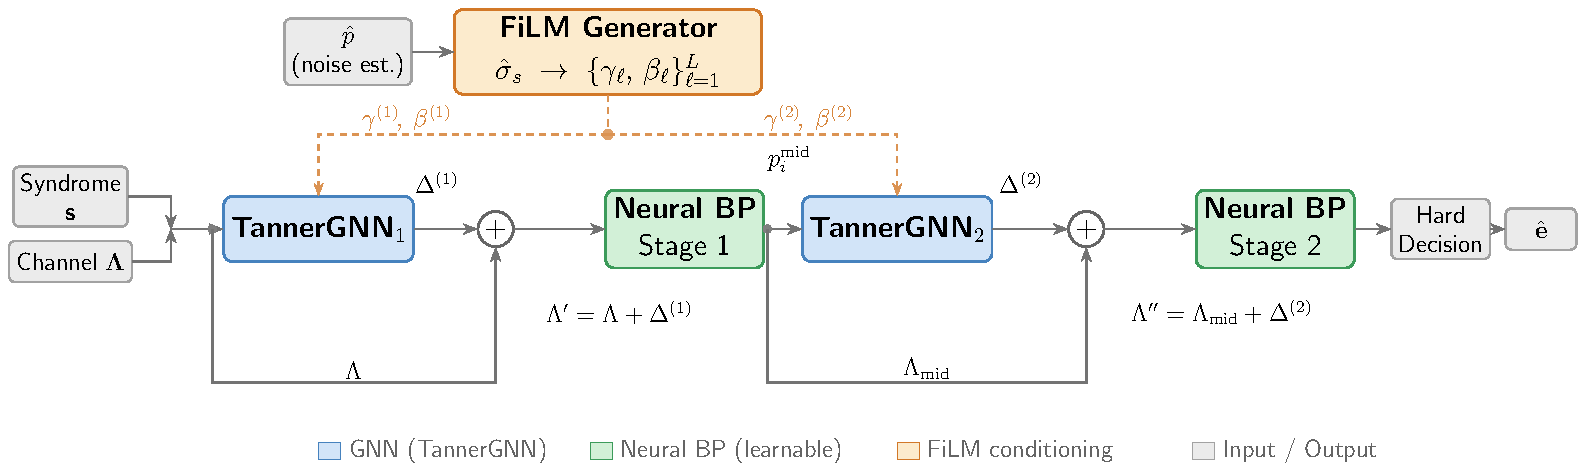
\includegraphics[width=\textwidth]{fig_interleaved_pipeline}
\caption{Interleaved GNN-BP pipeline. The GNN applies two successive
         LLR corrections: one before BP initialisation and one after
         $T_1$ iterations, using the mid-decoding posterior as an
         additional input. Both stages are trained end-to-end through
         the BP unroll.}
\label{fig:interleaved_pipeline}
\end{figure*}

\subsection{Training}\label{sec:training}

\begin{table}[t]
\centering
\caption{\DIFdelbeginFL \DIFdelFL{Architecture }\DIFdelendFL \DIFaddbeginFL \DIFaddFL{Configuration of the }\textsc{\DIFaddFL{TannerGNN}} \DIFaddFL{model behind
         Sec.~\ref{sec:gnn_positive} }\DIFaddendFL and \DIFdelbeginFL \DIFdelFL{training hyperparameters}\DIFdelendFL \DIFaddbeginFL \DIFaddFL{Sec.~\ref{sec:mismatch}}\DIFaddendFL .}
\label{tab:hparams}
\DIFdelbeginFL %DIFDELCMD < \resizebox{\columnwidth}{!}{%
%DIFDELCMD < \begin{tabular}{@{}ll@{}}
%DIFDELCMD < \toprule
%DIFDELCMD < \multicolumn{2}{@{}l}{\textit{GNN Architecture}} \\
%DIFDELCMD < \midrule
%DIFDELCMD < Hidden dimension $d_h$          & 64 \\
%DIFDELCMD < Message-passing layers $L$      & 3 \\
%DIFDELCMD < Edge types                      & 2 ($\Hmat_x$, $\Hmat_z$) \\
%DIFDELCMD < Node update                     & GRU \\
%DIFDELCMD < Node feature dim.               & 4 \\
%DIFDELCMD < FiLM conditioning               & 1 (scalar $\phat$) \\
%DIFDELCMD < Parameters                      & \makecell[l]{GNN-BP: 154k\\FiLM: 183k\\Interleaved: 183k} \\
%DIFDELCMD < \midrule
%DIFDELCMD < \multicolumn{2}{@{}l}{\textit{Training}} \\
%DIFDELCMD < \midrule
%DIFDELCMD < Optimizer                       & AdamW \\
%DIFDELCMD < Learning rate                   & $10^{-4}$ \\
%DIFDELCMD < Weight decay                    & $10^{-4}$ \\
%DIFDELCMD < Schedule                        & Cosine + 2-epoch warmup \\
%DIFDELCMD < Batch size                      & 16 \\
%DIFDELCMD < Focal loss $(\alpha,\gamma)$    & $(0.25,2.0)$ \\
%DIFDELCMD < Syndrome loss weight            & $0.1$ \\
%DIFDELCMD < BP iters (training / eval)      & 10 (flooding) / 100 \\
%DIFDELCMD < Best epoch                      & \makecell[l]{GNN-BP: 5 / 17\\FiLM: 18\\Interleaved: 1} \\
%DIFDELCMD < \midrule
%DIFDELCMD < \multicolumn{2}{@{}l}{\textit{Reference BP-OSD baseline}} \\
%DIFDELCMD < \midrule
%DIFDELCMD < \texttt{bp\_method}             & \texttt{ms} (min-sum) \\
%DIFDELCMD < \texttt{ms\_scaling\_factor}    & $0.8$ \\
%DIFDELCMD < \texttt{schedule}               & \texttt{serial} (layered) \\
%DIFDELCMD < \texttt{max\_iter}              & 100 \\
%DIFDELCMD < OSD (where used)                & \texttt{osd\_cs}, order 10 \\
%DIFDELCMD < \bottomrule
%DIFDELCMD < \end{tabular}}
%DIFDELCMD < %%%
\DIFdelendFL \DIFaddbeginFL \resizebox{\columnwidth}{!}{%
\begin{tabular}{@{}ll@{}}
\toprule
\multicolumn{2}{@{}l}{\textit{Architecture}} \\
\midrule
Message-passing layers / hidden width & 3 / 32 \\
Node features                         & 4 (value, one-hot node type) \\
Residual connections, layer norm      & yes \\
FiLM / attention                      & not used \\
Parameters                            & 39{,}329 \\
\midrule
\multicolumn{2}{@{}l}{\textit{Training}} \\
\midrule
Data & 8{,}000 shots, sinusoidal drift, $p\in[0.005,0.045]$ \\
Loss & focal, $\alpha=0.25$, $\gamma=2$, on $\mathbf{e}_z$ \\
Optimiser & AdamW, lr $2\times10^{-3}$, weight decay $10^{-4}$ \\
Batch size / epochs & 64 / 20, gradient clipping 1.0 \\
Checkpoint & lowest failures on 4{,}000 validation shots \\
Training seeds & 5 \\
\midrule
\multicolumn{2}{@{}l}{\textit{Decoders}} \\
\midrule
BP (training and Table~\ref{tab:gnn_flooding}) & flooding min-sum, scaling 0.8, 10 iter. \\
BP-OSD reference & serial min-sum, scaling 0.8, 100 iter., OSD-CS-10 \\
\bottomrule
\end{tabular}}
\DIFaddendFL \end{table}

\DIFdelbegin \DIFdel{Training uses }\DIFdelend \DIFaddbegin \paragraph{\DIFadd{Training loss.}} \DIFadd{For a shot with prior LLR
$\ell=\ln\bigl((1-p)/p\bigr)$ on every qubit, the GNN outputs a correction
$\delta_j$ for each qubit $j$, giving the corrected error probability
$q_j=\sigma\bigl(-(\ell+\delta_j)\bigr)$. The model is trained on the
}\DIFaddend focal loss~\cite{Lin2017Focal} \DIFaddbegin \DIFadd{against the true $Z$ error
$\mathbf{e}_z$,
}\begin{equation}
\DIFadd{\mathcal{L}=-\frac{1}{Bn}\sum_{b=1}^{B}\sum_{j=1}^{n}
\alpha_{t}\,(1-q_{t})^{\gamma}\log q_{t},
\label{eq:loss}
}\end{equation}
\DIFadd{where $q_t=q_j$ and $\alpha_t=\alpha$ if $e_{z,j}=1$, and
$q_t=1-q_j$ and $\alpha_t=1-\alpha$ otherwise, }\DIFaddend with \DIFdelbegin \DIFdel{$\alpha=0.25$,
$\gamma=2.0$ for class-imbalanced qubit errors, together with a syndrome
consistency term . The noise range is experiment dependent; in particular, the positive held-out result of }\DIFdelend \DIFaddbegin \DIFadd{$\alpha=0.25$ and $\gamma=2$. No syndrome-consistency term is used
for this model. At decoding time the corrected LLRs $\ell+\delta_j$ are
passed to both CSS components. The earlier FiLM and interleaved models
additionally used a syndrome-consistency term, the binary cross-entropy
between the measured syndrome and
$\tfrac12\bigl(1-\prod_{j\in\mathcal N(c)}(1-2q_j)\bigr)$ for each check
$c$ (weight $0.1$ in the configuration of the previous version).
}

\DIFadd{The training data and splits of the headline experiment are described in
}\DIFaddend Sec.~\ref{sec:gnn_positive}\DIFdelbegin \DIFdel{uses training
rates $p\in[0.02,0.03]$. \pending{Reconcile this with the earlier training
configuration $p\sim\mathrm{Uniform}[0.01,0.10]$ and report the data
range, number of samples per epoch, and checkpoint-selection rule for
each model variant.} Key hyperparameters are summarized }\DIFdelend \DIFaddbegin \DIFadd{; the configuration is summarised }\DIFaddend in
Table~\ref{tab:hparams}.

% ============================================================
%  IV. EXPERIMENTAL SETUP
% ============================================================
\section{Experimental Setup}\label{sec:setup}

\begin{figure*}[t]
\centering
\includegraphics[width=\textwidth]{fig_experimental_pipeline}
\caption{Experimental evaluation pipeline. Syndromes are sampled under
         static or drift noise models; each decoder receives identical
         syndrome batches to enable McNemar paired testing. Oracle
         experiments substitute true per-qubit rates for the uniform
         mean prior.}
\label{fig:experimental_pipeline}
\end{figure*}

\subsection{Evaluation regimes}\label{sec:regimes}

Two distinct evaluation regimes are used throughout this paper,
and the distinction is central to interpreting the results:

\textbf{Regime A (training-aligned baseline):} The GNN is evaluated
against flooding BP, the base decoder used during training. This
comparison isolates the gain relative to the decoder represented in the
training computation graph.

\textbf{Regime B (stronger classical baseline):} The same learned
correction is evaluated with the serial-schedule min-sum BP-OSD reference
configuration. This tests whether the correction also improves the
stronger classical decoder considered here; Sec.~\ref{sec:mismatch}
shows that it does not in the tested regime.

Unless otherwise stated, all experiments use $Z$-biased noise with
$\eta = 20$.

\subsection{Statistical protocol}\DIFaddbegin \label{sec:metrics}

\paragraph{\DIFadd{Logical failure.}}
\DIFadd{For each shot let $\hat{\mathbf{e}}_z$ and $\hat{\mathbf{e}}_x$ be the
decoder's hard decisions and let
$\mathbf{r}_z=\mathbf{e}_z\oplus\hat{\mathbf{e}}_z$ and
$\mathbf{r}_x=\mathbf{e}_x\oplus\hat{\mathbf{e}}_x$ be the residual
errors. A shot is counted as a logical failure if either
(i) the estimate does not reproduce the measured syndrome,
$\Hmat_x\hat{\mathbf{e}}_z\neq\mathbf{s}_x$ or
$\Hmat_z\hat{\mathbf{e}}_x\neq\mathbf{s}_z$; or
(ii) the syndrome is reproduced but the residual acts nontrivially on the
code space, $\mathbf{L}_x\mathbf{r}_z\neq\mathbf{0}$ or
$\mathbf{L}_z\mathbf{r}_x\neq\mathbf{0}$ over $\F_2$, where the rows of
$\mathbf{L}_x$ ($\mathbf{L}_z$) span the $k=12$ independent $X$-type
($Z$-type) logical operators modulo stabilizers. Condition (i) is required
because a syndrome-inconsistent residual is not a logical operator, so its
parity against a fixed set of logical representatives is not meaningful;
non-converged BP outputs are therefore always counted as failures. The
$X$- and $Z$-components are combined by logical OR, so the reported LER is
the probability that at least one of the 12 encoded qubits suffers a
logical error of any Pauli type in a single shot. At circuit level the same
rule is applied to the detector error model: a shot fails if the decoded
fault set does not reproduce the observed detection events, or if it does
and its predicted observable flips differ from the true ones.
}\DIFaddend 

For absolute LER comparisons we treat operating points with fewer than
100 observed logical-error events as preliminary; this is a reporting
heuristic rather than a formal power calculation. Decoder pairs are
evaluated on \emph{identical} syndrome samples, enabling paired
McNemar tests~\cite{McNemar1947}. We report Wilson score 95\% confidence
intervals for LER estimates.

\DIFdelbegin \DIFdel{Random seeds are fixed at $s=42$ for syndrome generation and $s+999$ for
validation splits. Unless otherwise stated,
the reported }\DIFdelend \DIFaddbegin \DIFadd{Training, validation and test data are drawn with distinct random seeds,
so no evaluation shot shares a random stream with a training shot, and
}\DIFaddend learned-decoder \DIFdelbegin \DIFdel{result is based on a single training seed; its confidence interval and
McNemar test therefore quantify test-set sampling uncertainty conditional
on that trained checkpoint, not training-to-training variability}\DIFdelend \DIFaddbegin \DIFadd{results are reported over five training seeds
(initialisation and minibatch order)}\DIFaddend . All training and evaluation used CPU
only; no GPU was available for this work. \DIFdelbegin \DIFdel{Representative per-epoch training times are $\sim\!17$\,s
(154k-parameter GNN-BP) and $\sim\!37$}\DIFdelend \DIFaddbegin \DIFadd{One training epoch of the
39k-parameter model of Sec.~\ref{sec:gnn_positive} takes about 16}\DIFaddend \,s \DIFdelbegin \DIFdel{(183k-parameter
interleaved model)}\DIFdelend \DIFaddbegin \DIFadd{on
four CPU cores}\DIFaddend .

% ============================================================
%  V. RESULTS
% ============================================================
\section{Results}\label{sec:results}

\subsection{Decoder configuration sensitivity}\label{sec:baseline}

Before presenting the GNN results, we quantify the sensitivity of the
classical baseline to decoder configuration. This sensitivity sets the
scale against which the learned-decoder results must be interpreted.

\begin{table*}[t]
\centering
\caption{Effect of BP-OSD configuration on $\code{288}{12}{18}$, $p=0.04$,
         $\eta=20$, \DIFdelbeginFL \DIFdelFL{5}%DIFDELCMD < {%%%
\DIFdelFL{,}%DIFDELCMD < }%%%
\DIFdelFL{000 }\DIFdelendFL \DIFaddbeginFL \DIFaddFL{$100{,}000$ }\DIFaddendFL identical shots\DIFaddbeginFL \DIFaddFL{, separate-CSS decoding with
         priors $p_Z=p\eta/(\eta+1)$, $p_X=p/(\eta+1)$}\DIFaddendFL . \DIFdelbeginFL \DIFdelFL{CIs }\DIFdelendFL \DIFaddbeginFL \DIFaddFL{95\% Wilson intervals
         }\DIFaddendFL in brackets. \DIFaddbeginFL \DIFaddFL{OSD is OSD-CS of order 10.}\DIFaddendFL }
\label{tab:smoking_gun}
\begin{tabular}{@{}llllcc@{}}
\toprule
Config & Schedule & Method & Iter & LER & Errors \\
\midrule
\DIFdelbeginFL \DIFdelFL{Original }\DIFdelendFL BP              & parallel & prod-sum & 30  & \DIFdelbeginFL \DIFdelFL{0.0506 }\DIFdelendFL \DIFaddbeginFL \DIFaddFL{0.0569 }\DIFaddendFL [\DIFdelbeginFL \DIFdelFL{0.045, 0.057}\DIFdelendFL \DIFaddbeginFL \DIFaddFL{0.0555, 0.0583}\DIFaddendFL ] & \DIFdelbeginFL \DIFdelFL{253 }\DIFdelendFL \DIFaddbeginFL \DIFaddFL{5}{\DIFaddFL{,}}\DIFaddFL{689 }\DIFaddendFL \\
\DIFdelbeginFL \DIFdelFL{Reference }\DIFdelendFL BP              & serial   & ms(0.8)  & 100 & \DIFdelbeginFL \DIFdelFL{0.0014 }\DIFdelendFL \DIFaddbeginFL \DIFaddFL{0.00174 }\DIFaddendFL [\DIFdelbeginFL \DIFdelFL{0.001, 0.003}\DIFdelendFL \DIFaddbeginFL \DIFaddFL{0.00150, 0.00202}\DIFaddendFL ] & \DIFdelbeginFL \DIFdelFL{7 }\DIFdelendFL \DIFaddbeginFL \DIFaddFL{174 }\DIFaddendFL \\
\DIFdelbeginFL \DIFdelFL{Original }\DIFdelendFL BP-OSD          & parallel & prod-sum & 30  & \DIFdelbeginFL \DIFdelFL{0.0346 }\DIFdelendFL \DIFaddbeginFL \DIFaddFL{0.0398 }\DIFaddendFL [\DIFdelbeginFL \DIFdelFL{0.030, 0.040}\DIFdelendFL \DIFaddbeginFL \DIFaddFL{0.0386, 0.0411}\DIFaddendFL ] & \DIFdelbeginFL \DIFdelFL{173 }\DIFdelendFL \DIFaddbeginFL \DIFaddFL{3}{\DIFaddFL{,}}\DIFaddFL{983 }\DIFaddendFL \\
\DIFdelbeginFL \DIFdelFL{Ref.\ }\DIFdelendFL BP-OSD          & serial   & ms(0.8)  & 100 & \DIFdelbeginFL \DIFdelFL{0.0002 }\DIFdelendFL \DIFaddbeginFL \DIFaddFL{0.00034 }\DIFaddendFL [\DIFdelbeginFL \DIFdelFL{0.000, 0.001}\DIFdelendFL \DIFaddbeginFL \DIFaddFL{0.00024, 0.00048}\DIFaddendFL ] & \DIFdelbeginFL \DIFdelFL{1 }\DIFdelendFL \DIFaddbeginFL \DIFaddFL{34 }\DIFaddendFL \\
\bottomrule
\end{tabular}
\end{table*}

Table~\ref{tab:smoking_gun} illustrates how strongly decoder
configuration changes the finite-length result \DIFdelbegin \DIFdel{. In the 5}%DIFDELCMD < {%%%
\DIFdel{,}%DIFDELCMD < }%%%
\DIFdel{000-shot
pilot, the original parallel }\DIFdelend \DIFaddbegin \DIFadd{on $100{,}000$ identical
shots. Parallel }\DIFaddend product-sum BP-OSD \DIFdelbegin \DIFdel{configuration reduces
LER from $0.0506$ to $0.0346$ relative to }\DIFdelend \DIFaddbegin \DIFadd{with 30 iterations lowers the LER of }\DIFaddend the
corresponding plain BP \DIFdelbegin \DIFdel{,
but remains far worse than the serial min-sum configurations. The
reference }\DIFdelend \DIFaddbegin \DIFadd{only from $0.0569$ to $0.0398$, whereas }\DIFaddend serial
min-sum \DIFdelbegin \DIFdel{BP-OSD produces only one logical error in this
sample, so the value $0.0002$ should be interpreted as a preliminary
estimate rather than a precisely resolved LER}\DIFdelend \DIFaddbegin \DIFadd{BP with 100 iterations reaches $0.0017$ without OSD and $0.00034$
with it, more than two orders of magnitude below the parallel
product-sum configurations}\DIFaddend .

A separate \DIFdelbegin \DIFdel{$N=100{,}000$}\DIFdelend \DIFaddbegin \DIFadd{$100{,}000$}\DIFaddend -shot experiment \DIFdelbegin \DIFdel{is shown in
}\DIFdelend \DIFaddbegin \DIFadd{(}\DIFaddend Fig.~\ref{fig:baseline_decomp}\DIFdelbegin \DIFdel{. In that experiment, changing to }\DIFdelend \DIFaddbegin \DIFadd{)
changes one factor at a time. The flooding comparator is min-sum BP with
scaling factor $0.8$, at most 100 iterations, stopping at the first
iteration whose hard decision satisfies the syndrome, with a parallel
(flooding) schedule; the second decoder is identical except for }\DIFaddend the serial
schedule\DIFdelbegin \DIFdel{and then adding }\DIFdelend \DIFaddbegin \DIFadd{; the third adds }\DIFaddend OSD-CS-10\DIFdelbegin \DIFdel{yields an overall
approximately $40\times$ reduction relative to the flooding comparator.
\pending{State the exact BP method, scaling factor, iteration count, and
stopping rule for the 100k flooding comparator. These must match the
serial configuration except for the factor being isolated; otherwise the
$6.7\times$ schedule decomposition is confounded.}
}\DIFdelend \DIFaddbegin \DIFadd{. The logical error rate falls from
$1.28\times10^{-2}$ to $1.45\times10^{-3}$ ($8.8\times$, paired
$n_{10}/n_{01}=1138/3$) and then to $2.7\times10^{-4}$ ($5.4\times$,
$118/0$), about $47\times$ overall.
}\DIFaddend 

\begin{figure}[t]
\centering
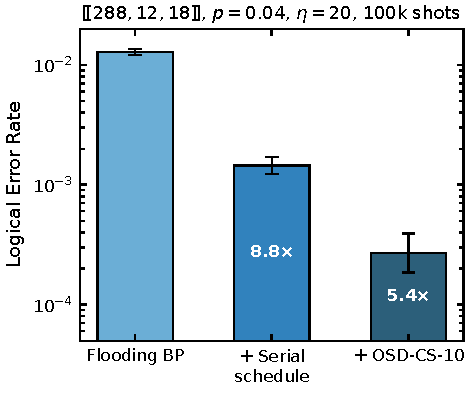
\includegraphics[width=\columnwidth]{fig_F1_baseline_decomp}
\caption{Baseline decomposition on $\code{288}{12}{18}$, $p=0.04$,
         $\eta=20$, 100k \DIFaddbeginFL \DIFaddFL{identical }\DIFaddendFL shots. \DIFdelbeginFL \DIFdelFL{The figure is intended to isolate the
         effect of serial scheduling }\DIFdelendFL \DIFaddbeginFL \DIFaddFL{Min-sum BP (scaling 0.8, at most
         100 iterations) with flooding }\DIFaddendFL and \DIFdelbeginFL \DIFdelFL{subsequent OSD-CS-10}\DIFdelendFL \DIFaddbeginFL \DIFaddFL{then serial schedule, then serial
         BP-OSD-CS-10. Bars: LER with 95\% Wilson intervals}\DIFaddendFL ; \DIFaddbeginFL \DIFaddFL{labels give }\DIFaddendFL the
         \DIFdelbeginFL \DIFdelFL{exact
         flooding-BP comparator configuration must be reported in the
         text before the multiplicative factors are interpreted causally}\DIFdelendFL \DIFaddbeginFL \DIFaddFL{factor gained at each step}\DIFaddendFL .}
\label{fig:baseline_decomp}
\end{figure}

These data do not identify a universally optimal configuration. They do
show that schedule, update rule, iteration budget, and post-processing
can dominate the measured finite-length LER. Learned-decoder comparisons
must therefore specify and control these parameters.

\subsection{Uniform-prior scaling invariance of min-sum BP}\label{sec:invariance}

\begin{proposition}[Uniform positive-scaling invariance]\label{prop:invariance}
Consider separate-CSS min-sum BP with no message clipping or offset. If
all channel LLRs in one CSS component are multiplied by the same factor
$a>0$, then every BP message and posterior LLR is multiplied by $a$ at
every iteration. Consequently, all hard decisions are unchanged.
\end{proposition}

\begin{proof}
At initialization, each variable-to-check message is proportional to the
corresponding channel LLR and therefore scales by $a$. Assume all
variable-to-check messages at iteration $t$ have scaled by $a$. The
syndrome factor $(-1)^{s_j}$ in Eq.~\eqref{eq:ctv} is unchanged, the sign
of every message is unchanged because $a>0$, and
$\min_i a|x_i|=a\min_i|x_i|$. Hence every check-to-variable message also
scales by $a$. Equation~\eqref{eq:vtc} then shows that the next
variable-to-check messages scale by $a$. Induction establishes the claim
for all iterations and for the final posterior LLRs.
\end{proof}

For a uniform channel prior, replacing a common positive LLR $\Lambda$
by another positive value $\Lambda'$ is equivalent to the scaling
$a=\Lambda'/\Lambda$. The proposition explains why changing only the assumed uniform physical
error rate cannot change hard decisions of ideal min-sum BP. Clipping, offsets, damping rules that depend on
magnitude, non-uniform priors, or sum-product updates can break the exact
scaling argument.

We \DIFdelbegin \DIFdel{observed the expected invariance in the implemented decoder:
$1{,}740/1{,}740$ bit-identical outputs when }\DIFdelend \DIFaddbegin \DIFadd{checked the proposition on 2}{\DIFadd{,}}\DIFadd{000 shots each. With ldpc min-sum BP
(serial or flooding, 100 iterations), }\DIFaddend changing the assumed \DIFdelbegin \DIFdel{prior
}\DIFdelend \DIFaddbegin \DIFadd{uniform rate
}\DIFaddend from $p=0.015$ to \DIFdelbegin \DIFdel{$p=0.0286$ }\DIFdelend \DIFaddbegin \DIFadd{$0.0286$ }\DIFaddend on $\code{288}{12}{18}$, \DIFdelbegin \DIFdel{and
$1{,}000/1{,}000$ bit-identical outputs for $p=0.04$ versus $p=0.02$ in
the tested }\DIFdelend \DIFaddbegin \DIFadd{or from $0.04$ to
$0.02$ on $\code{72}{12}{6}$, leaves every hard decision unchanged
(2}{\DIFadd{,}}\DIFadd{000/2}{\DIFadd{,}}\DIFadd{000), and an assumed-bias sweep
$\eta\in\{1,2,5,10,20,50,100\}$ at $p=0.03$ gives identical decisions at
every value. Two cases fall outside the proposition, and the invariance
fails there: our PyTorch }\DIFaddend min-sum \DIFdelbegin \DIFdel{setting. The same 1}\DIFdelend \DIFaddbegin \DIFadd{implementation clamps messages to
$\pm20$ and changes 18/2}\DIFaddend {,}\DIFdelbegin \DIFdel{000-shot test was also identical
for the tested }\DIFdelend \DIFaddbegin \DIFadd{000 decisions on $\code{288}{12}{18}$, and
}\DIFaddend sum-product \DIFdelbegin \DIFdel{configuration; because Proposition~\ref{prop:invariance}
does not apply to the tanh nonlinearity,we report that observation as
empirical rather than structural.
}\DIFdelend \DIFaddbegin \DIFadd{BP changes 25--43 of 2}{\DIFadd{,}}\DIFadd{000.
}\DIFaddend 

\begin{remark}[What the proposition does and does not imply]
The result applies to the BP pathway when adaptivity enters only by
changing a uniform channel-prior magnitude. It does \emph{not} establish
that a global conditioning scalar is information-theoretically useless
to a GNN: a learned model could combine a global noise estimate with
local syndrome structure and change its nonlinear decision rule. The experiments below test a narrower hypothesis: spatially resolved
per-qubit calibration can change the relative reliabilities seen by the
decoder, whereas a single graph-wide scalar cannot provide that spatial
information.
\end{remark}

\subsection{GNN improvement over flooding BP}\label{sec:gnn_positive}

We evaluated the GNN against flooding \DIFdelbegin \DIFdel{BP---the }\DIFdelend \DIFaddbegin \DIFadd{BP, the }\DIFaddend decoder it was trained
\DIFdelbegin \DIFdel{against---on }\DIFdelend \DIFaddbegin \DIFadd{against. The training set is }\DIFaddend 8{,}000 \DIFdelbegin \DIFdel{held-out syndromes.
}\DIFdelend \DIFaddbegin \DIFadd{shots from two sinusoidally drifting
streams, $p(t)=p_0+0.015\sin(2\pi t/500)$ with $p_0\in\{0.02,0.03\}$, so
the training rates span $p\in[0.005,0.045]$. Validation (4}{\DIFadd{,}}\DIFadd{000 shots at
$p=0.04$) and test sets (20}{\DIFadd{,}}\DIFadd{000 shots at $p=0.04$, inside the training
range; 10}{\DIFadd{,}}\DIFadd{000 shots at $p=0.06$, outside it) are drawn with separate
random seeds. The checkpoint is chosen by the lowest validation failure
count over 20 epochs, each test set is scored once on that checkpoint, and
training is repeated with five seeds (Table~\ref{tab:hparams}).
}\DIFaddend 

\begin{table}[t]
\centering
\DIFdelbeginFL %DIFDELCMD < \caption{%
{%DIFAUXCMD
\DIFdelFL{GNN-BP vs.\ flooding BP on $\code{72}{12}{6}$, $\eta=20$,
         8}%DIFDELCMD < {%%%
\DIFdelFL{,}%DIFDELCMD < }%%%
\DIFdelFL{000 held-out test syndromes. GNN trained for 20 epochs
         on separate 8}%DIFDELCMD < {%%%
\DIFdelFL{,}%DIFDELCMD < }%%%
\DIFdelFL{000 training syndromes at $p\in[0.02,0.03]$.
         Best checkpoint at epoch 5 by validation LER.}}
%DIFAUXCMD
\DIFdelendFL \DIFaddbeginFL \caption{\DIFaddFL{GNN-BP vs.\ flooding BP on $\code{72}{12}{6}$, $\eta=20$, five training seeds (mean $\pm$ s.d.).
Failures follow the definition in Sec.~\ref{sec:metrics}.
95\% Wilson intervals for single decoders are $\pm0.004$ at $p=0.04$
and $\pm0.009$ at $p=0.06$.}}
\DIFaddendFL \label{tab:gnn_flooding}
\DIFdelbeginFL %DIFDELCMD < \resizebox{\columnwidth}{!}{%
%DIFDELCMD < \begin{tabular}{@{}lcccc@{}}
%DIFDELCMD < \toprule
%DIFDELCMD <  & Flooding BP & GNN-BP & $n_{10}$ / $n_{01}$ & McNemar $p$ \\
%DIFDELCMD < \midrule
%DIFDELCMD < $p=0.04$, ep. 5 & 0.0990 & 0.0838 & 170 / 48 & $\approx 0$ \\
%DIFDELCMD < $p=0.04$, ep. 1 & 0.0990 & 0.0975 & 91 / 79  & 0.399 \\
%DIFDELCMD < \bottomrule
%DIFDELCMD < \end{tabular}}
%DIFDELCMD < %%%
\DIFdelendFL \DIFaddbeginFL \resizebox{\columnwidth}{!}{%
\begin{tabular}{@{}lcc@{}}
\toprule
Decoder & $p=0.04$ ($20$k shots) & $p=0.06$ ($10$k shots)\\
\midrule
BP, 10 iter. & 0.1077 & 0.2867\\
GNN + BP, 10 iter. & $0.0942\pm0.0006$ & $0.2564\pm0.0019$\\
\quad relative reduction & $12.5\%\pm0.6\%$ & $10.6\%\pm0.7\%$\\
\quad McNemar $n_{10}/n_{01}$ (range) & 313--370 / 64--95 & 343--394 / 66--80\\
BP, 100 iter. & 0.0863 & 0.2403\\
Serial BP-OSD-CS(10), 100 iter. & 0.0707 & 0.2138\\
\bottomrule
\end{tabular}}
\DIFaddendFL \end{table}

\DIFdelbegin \DIFdel{Table~\ref{tab:gnn_flooding} gives the primary learned-decoder result. At the epoch-5 checkpoint, GNN-BP reduces LER by $15.4\%$ relative to
flooding BP on 8}%DIFDELCMD < {%%%
\DIFdel{,}%DIFDELCMD < }%%%
\DIFdel{000 held-out syndromes }\DIFdelend \DIFaddbegin \DIFadd{GNN pre-processing reduces the failure rate of 10-iteration BP by
$12.5\%\pm0.6\%$ }\DIFaddend at $p=0.04$ \DIFdelbegin \DIFdel{($n_{10}=170$,$n_{01}=48$, McNemar $\chi^2=67.16$,$p<10^{-15}$) . The test point }\DIFdelend \DIFaddbegin \DIFadd{and $10.6\%\pm0.7\%$ at $p=0.06$, which }\DIFaddend lies
outside the training range\DIFdelbegin \DIFdel{$p\in[0.02,0.03]$, so the result demonstrates transfer to a higher
physical error rate for this checkpoint. Because only one training seed
is reported,we do not interpret the paired test as evidence for
training-to-training reproducibility.
A }\DIFdelend \DIFaddbegin \DIFadd{; every seed is significant
($p<10^{-36}$, McNemar). The gain comes mostly from convergence: shots where
BP fails to reproduce the syndrome fall from 1}{\DIFadd{,}}\DIFadd{740 to 838--975 of 20}{\DIFadd{,}}\DIFadd{000.
The gain does not close the gap to longer decoding: 100-iteration BP (0.0863)
and serial BP-OSD (0.0707) both outperform GNN + 10-iteration BP.
}

\DIFadd{On the original single-seed checkpoint, a }\DIFaddend gradient audit found non-zero
signal through the network (input-to-readout gradient ratio $0.22$) and
non-trivial LLR corrections (mean $|\Delta_i|=0.854$).

A fixed-dataset capacity test provides an additional diagnostic: a GNN
trained on 1{,}000 fixed syndromes for 50 epochs \DIFdelbegin \DIFdel{achieved a $14\%$ LER
reduction }\DIFdelend \DIFaddbegin \DIFadd{reduced the failure count
}\DIFaddend on those same syndromes \DIFdelbegin \DIFdel{(McNemar $p=0.004$, $n_{10}=17$}\DIFdelend \DIFaddbegin \DIFadd{from 105 to 93 ($11\%$; $n_{10}=15$}\DIFaddend , $n_{01}=3$\DIFaddbegin \DIFadd{,
McNemar $p=0.0095$}\DIFaddend ). This experiment tests the ability of the architecture and
optimizer to fit the supplied examples; it is not a generalization
result. The interleaved \DIFdelbegin \DIFdel{model reached its best validation checkpoint at
epoch 1 and did not train successfully, so no performance conclusion
about that architecture is drawn from the current run (see Limitations)}\DIFdelend \DIFaddbegin \DIFadd{architecture of Sec.~\ref{sec:neuralbp} is not evaluated in this work}\DIFaddend .


\DIFdelbegin %DIFDELCMD < \begin{figure}[t]
%DIFDELCMD < \centering
%DIFDELCMD < \includegraphics[width=\columnwidth]{fig_F5_interleaved_training}
%DIFDELCMD < %%%
%DIFDELCMD < \caption{%
{%DIFAUXCMD
\DIFdelFL{Interleaved model training curves (183k parameters).
         The best validation checkpoint occurs at epoch~1 and the
         validation loss increases thereafter. The current run does
         not provide a trained interleaved decoder for comparison.}}
%DIFAUXCMD
%DIFDELCMD < \label{fig:interleaved_training}
%DIFDELCMD < \end{figure}
%DIFDELCMD < 

%DIFDELCMD < %%%
\DIFdelend \subsection{Training/evaluation baseline mismatch}\label{sec:mismatch}

Although the GNN improves flooding BP, the same correction does not
improve the serial min-sum BP-OSD reference configuration. \DIFdelbegin \DIFdel{Note that Tables~\ref{tab:gnn_flooding}
and ~\ref{tab:gnn_null} report different evaluation regimes
(Regime~A and Regime~B of Sec.~\ref{sec:regimes})on different
syndrome sets , and their LER values are not directly comparable:
}\DIFdelend \DIFaddbegin \DIFadd{We pass the
corrected LLRs of each of the five trained models to BP-OSD and compare
with BP-OSD alone on 20}{\DIFadd{,}}\DIFadd{000 identical fresh shots per error rate
(Table~\ref{tab:gnn_null}); these shots differ from the test sets of
Table~\ref{tab:gnn_flooding}.
}\DIFaddend 

\begin{table}[t]
\centering
\caption{\DIFdelbeginFL \DIFdelFL{GNN-BP }\DIFdelendFL \DIFaddbeginFL \DIFaddFL{GNN+OSD }\DIFaddendFL vs.\ serial BP-OSD on $\code{72}{12}{6}$, $\eta=20$,
         \DIFdelbeginFL \DIFdelFL{8}%DIFDELCMD < {%%%
\DIFdelFL{,}%DIFDELCMD < }%%%
\DIFdelFL{000 }\DIFdelendFL \DIFaddbeginFL \DIFaddFL{$20{,}000$ identical }\DIFaddendFL shots \DIFaddbeginFL \DIFaddFL{per $p$, five GNN training seeds}\DIFaddendFL .
         \DIFdelbeginFL \DIFdelFL{Decoders evaluated on identical syndromes}\DIFdelendFL \DIFaddbeginFL \DIFaddFL{Serial min-sum BP-OSD-CS-10 (scaling 0.8, 100 iterations)}\DIFaddendFL .}
\label{tab:gnn_null}
\DIFdelbeginFL %DIFDELCMD < \resizebox{\columnwidth}{!}{%
%DIFDELCMD < \begin{tabular}{@{}lcccl@{}}
%DIFDELCMD < \toprule
%DIFDELCMD < $p$ & Serial BP-OSD & GNN+OSD & $p_\mathrm{McN}$ & Verdict \\
%DIFDELCMD < \midrule
%DIFDELCMD < 0.020 & 0.0046 & 0.0050 & 0.68 & tie \\
%DIFDELCMD < 0.030 & 0.0377 & 0.0399 & 0.63 & tie \\
%DIFDELCMD < 0.040 & 0.0831 & 0.0876 & 0.033 & GNN \emph{worse} \\
%DIFDELCMD < 0.050 & 0.1515 & 0.1555 & $3.6\!\times\!10^{-5}$ & GNN \emph{worse} \\
%DIFDELCMD < \bottomrule
%DIFDELCMD < \end{tabular}}
%DIFDELCMD < %%%
\DIFdelendFL \DIFaddbeginFL \resizebox{\columnwidth}{!}{%
\begin{tabular}{@{}lccc@{}}
\toprule
$p$ & Serial BP-OSD & GNN+OSD (5 seeds) & Seeds worse ($p_\mathrm{McN}<0.05$) \\
\midrule
0.02 & 0.0093 & 0.0095--0.0102 & 1/5 \\
0.03 & 0.0297 & 0.0306--0.0317 & 5/5 \\
0.04 & 0.0676 & 0.0688--0.0709 & 4/5 \\
0.05 & 0.1354 & 0.1384--0.1418 & 5/5 \\
\bottomrule
\end{tabular}}
\DIFaddendFL \end{table}

\begin{figure}[t]
\centering
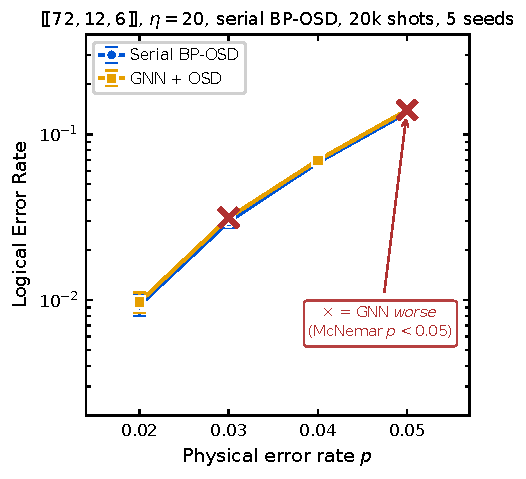
\includegraphics[width=\columnwidth]{fig_F4_phase4_ler}
\caption{GNN+OSD vs.\ serial BP-OSD LER on $\code{72}{12}{6}$,
         $\eta=20$, \DIFdelbeginFL \DIFdelFL{8}\DIFdelendFL \DIFaddbeginFL \DIFaddFL{20}\DIFaddendFL {,}000 shots \DIFaddbeginFL \DIFaddFL{per point; GNN+OSD is the mean over
         five training seeds}\DIFaddendFL . Red $\times$ marks operating points where
         \DIFdelbeginFL \DIFdelFL{GNN }\DIFdelendFL \DIFaddbeginFL \DIFaddFL{every seed }\DIFaddendFL is statistically worse (McNemar $p<0.05$).
         Wilson 95\% CI error bars.}
\label{fig:gnn_null_curve}
\end{figure}

Table~\ref{tab:gnn_null} and Fig.~\ref{fig:gnn_null_curve} show that the
GNN-corrected decoder \DIFdelbegin \DIFdel{is statistically indistinguishable from }\DIFdelend \DIFaddbegin \DIFadd{never improves on }\DIFaddend serial BP-OSD\DIFdelbegin \DIFdel{at the two lower error rates and }\DIFdelend \DIFaddbegin \DIFadd{: at $p=0.02$ only one
seed of five is significantly worse, and from $p=0.03$ on 14 of 15
seed--error-rate pairs are }\DIFaddend significantly \emph{worse}\DIFdelbegin \DIFdel{at
the two higher rates}\DIFdelend . The same \DIFdelbegin \DIFdel{checkpoint improves }\DIFdelend \DIFaddbegin \DIFadd{checkpoints
improve }\DIFaddend flooding BP, so \DIFdelbegin \DIFdel{these
data show that }\DIFdelend the learned correction does not transfer unchanged
to the stronger decoder.

\DIFdelbegin \DIFdel{The experiment establishes a transfer failure }\DIFdelend \DIFaddbegin \begin{table}[t]
\centering
\caption{\DIFaddFL{Paired failure sets on $\code{72}{12}{6}$, $p=0.04$, $\eta=20$,
         $20{,}000$ identical held-out shots. BP: 10-iteration flooding
         min-sum (the GNN's training decoder). GNN rows give the range over
         five training seeds. ``Non-conv.'': the estimate does not reproduce
         the syndrome.}}
\label{tab:failure_sets}
\resizebox{\columnwidth}{!}{%
\begin{tabular}{@{}lcc@{}}
\toprule
Decoder & Failures & Non-conv. \\
\midrule
BP, 10 iter.            & 2{,}155 & 1{,}740 \\
BP, 100 iter.           & 1{,}727 & 700 \\
Serial BP-OSD           & 1{,}414 & 0 \\
GNN + BP, 10 iter.      & 1{,}874--1{,}906 & 838--975 \\
GNN + BP-OSD            & 1{,}439--1{,}451 & 0 \\
\midrule
\multicolumn{3}{@{}l}{\textit{Overlaps}} \\
BP-OSD failures that BP also fails & \multicolumn{2}{c}{1{,}319 / 1{,}414 (93\%)} \\
BP-100 failures that BP also fails & \multicolumn{2}{c}{1{,}727 / 1{,}727 (100\%)} \\
Shots GNN fixes for BP (BP fails, GNN+BP succeeds) & \multicolumn{2}{c}{313--370} \\
\quad of which BP did not converge & \multicolumn{2}{c}{91--93\%} \\
\quad of which BP-OSD also fails & \multicolumn{2}{c}{31--36\%} \\
BP-OSD failures that GNN+BP also fails & \multicolumn{2}{c}{87--88\%} \\
GNN+BP-OSD vs.\ BP-OSD: newly failed / rescued & \multicolumn{2}{c}{237--282 / 206--254} \\
\quad newly failed shots that BP also fails & \multicolumn{2}{c}{91--95\%} \\
\bottomrule
\end{tabular}}
\end{table}

\DIFadd{Table~\ref{tab:failure_sets} compares the failure sets of all decoders on
identical shots. The failure sets are nested rather than disjoint: every
shot that 100-iteration BP fails is also failed by 10-iteration BP, and
93\% of BP-OSD's failures are BP failures. What separates the decoders is
mainly convergence: 81\% of 10-iteration BP failures are shots on which BP
does not reach a syndrome-consistent estimate, whereas BP-OSD always
returns one. No decoder fails on any error of weight $\le 2=(d-1)/2$;
all failures involve errors of weight at least 3 (mean weight 5.4--5.7).
In 1}{\DIFaddend ,\DIFdelbegin \DIFdel{but it does not by itself
identify the residual-failure mechanism.
}\DIFdelend \DIFaddbegin }\DIFadd{411 of BP-OSD's 1}{\DIFadd{,}}\DIFadd{414 failures the returned correction is
syndrome-consistent and no heavier than the true error, so these failures
are limited by the code and the noise, not by a decoder returning an
unnecessarily heavy estimate.
}

\DIFadd{The GNN's gains lie where BP-OSD already succeeds. Of the 313--370 shots
the GNN fixes for 10-iteration BP, 91--93\% are shots on which BP did not
converge, and only 31--36\% are shots that BP-OSD fails; conversely,
GNN+BP still fails 87--88\% of BP-OSD's failures. When the same
corrections are passed to BP-OSD, they reshuffle rather than remove its
failures (237--282 newly failed vs.\ 206--254 rescued shots), almost
entirely among the hard shots on which BP itself fails. They also make
OSD return heavier incorrect estimates (20--43 failures with an estimate
heavier than the true error, vs.\ 3 for BP-OSD alone). The same pattern
holds at $p=0.06$ (10}{\DIFadd{,}}\DIFadd{000 shots): 96\% of BP-OSD failures are BP
failures, and 30--36\% of the GNN's fixes are BP-OSD failures.
}

\DIFaddend The GNN was optimized through a 10-iteration flooding-BP computation graph
and is then inserted ahead of a decoder with a different schedule,
iteration budget, and OSD post-processing. \DIFdelbegin \DIFdel{The experiment therefore does not establish that LLR
corrections learned through the flooding-BP computation graph remain
useful after the schedule, iteration budget, and post-processing are
changed. At the same time,
claims that the two decoders fail on ``structurally different'' trapping
sets require an explicit paired failure-overlap or trapping-set analysis,
which is not included here. \pending{If available, add the Jaccard/overlap
statistics of the two failure sets and classify representative failures;
otherwise keep the explanation at the level of training/evaluation
mismatch.} }\DIFdelend Training directly against the
target decoder, or against a differentiable surrogate of its
post-processing stage, remains the appropriate test of whether learned
augmentation can improve BP-OSD.

\subsection{Per-qubit calibration gap}\label{sec:oraclegap}

Under spatially non-uniform per-qubit noise\DIFdelbegin \DIFdel{($p_i \sim
\mathrm{LogNormal}(\log p_\mathrm{mean}, \sigma)$, fresh per shot )}\DIFdelend , \DIFdelbegin \DIFdel{a }\DIFdelend \DIFaddbegin \DIFadd{each data qubit has rate
$p_i=p\,e^{\sigma z_i-\sigma^2/2}$ with $z_i\sim\mathcal N(0,1)$ drawn
fresh every shot (capped at 0.5), so the mean rate is $p$ for every
$\sigma$; the mean-prior decoder uses the uniform rate $p$. A }\DIFaddend decoder knowing the true per-qubit rates
\DIFdelbegin \DIFdel{substantially outperforms
a }\DIFdelend \DIFaddbegin \DIFadd{(serial min-sum BP-OSD-CS-10 with the true $p_i$ as priors) substantially
outperforms the }\DIFaddend mean-prior decoder.

\begin{figure}[t]
\centering
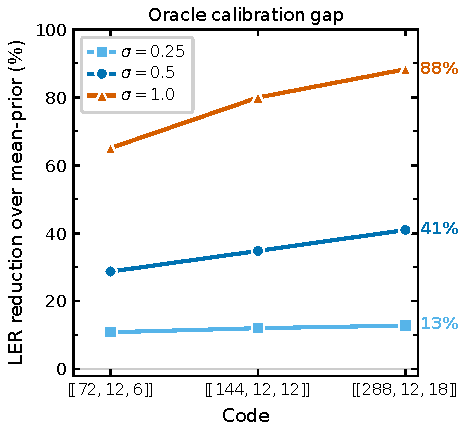
\includegraphics[width=\columnwidth]{fig_F2_oracle_vs_distance}
\caption{Oracle calibration gap (percentage LER reduction \DIFdelbeginFL \DIFdelFL{from
         per-qubit vs.\ }\DIFdelendFL \DIFaddbeginFL \DIFaddFL{of
         per-qubit-oracle over }\DIFaddendFL mean-prior BP-OSD)\DIFdelbeginFL \DIFdelFL{at $\sigma=1.0$}\DIFdelendFL , 50k \DIFaddbeginFL \DIFaddFL{identical }\DIFaddendFL shots \DIFdelbeginFL \DIFdelFL{($\code{72}{12}{6}$, $\code{144}{12}{12}$)
         and 30k shots ($\code{288}{12}{18}$)}\DIFdelendFL \DIFaddbeginFL \DIFaddFL{per
         point}\DIFaddendFL . Operating points: $p=0.04$, $0.06$, $0.07$ \DIFdelbeginFL \DIFdelFL{respectively}\DIFdelendFL \DIFaddbeginFL \DIFaddFL{for the three
         codes}\DIFaddendFL ; cross-code comparisons are partially confounded by the
         differing operating points.}
\label{fig:oracle_gap}
\end{figure}

\begin{table*}[t]
\centering
\caption{Oracle gap: percentage LER reduction \DIFdelbeginFL \DIFdelFL{from per-qubit
         }\DIFdelendFL \DIFaddbeginFL \DIFaddFL{of per-qubit-oracle }\DIFaddendFL over
         mean-prior \DIFdelbeginFL \DIFdelFL{BP-OSD}\DIFdelendFL \DIFaddbeginFL \DIFaddFL{serial BP-OSD-CS-10, $50{,}000$ identical shots per
         cell. Parentheses: mean-prior failures}\DIFaddendFL . \DIFdelbeginFL \DIFdelFL{All }\DIFdelendFL McNemar
         \DIFdelbeginFL \DIFdelFL{$p \ll 10^{-3}$}\DIFdelendFL \DIFaddbeginFL \DIFaddFL{$p<10^{-20}$ in the upper three rows and $p<10^{-5}$ in the last}\DIFaddendFL .
         \DIFdelbeginFL \DIFdelFL{Parenthetical counts are mean-prior error events}\DIFdelendFL \DIFaddbeginFL \DIFaddFL{The upper three rows use the operating points of
         Fig.~\ref{fig:oracle_gap}; the last row fixes $p=0.04$}\DIFaddendFL .}
\label{tab:oracle}
\DIFdelbeginFL %DIFDELCMD < \begin{tabular}{@{}lccc@{}}
%DIFDELCMD < %%%
\DIFdelendFL \DIFaddbeginFL \begin{tabular}{@{}llccc@{}}
\DIFaddendFL \toprule
Code ($d$) & \DIFaddbeginFL \DIFaddFL{$p$ }& \DIFaddendFL $\sigma=0.25$ & $\sigma=0.5$ & $\sigma=1.0$ \\
\midrule
$\code{72}{12}{6}$   (6)  & \DIFdelbeginFL \DIFdelFL{$+11\%$ (3457}\DIFdelendFL \DIFaddbeginFL \DIFaddFL{0.04 }& \DIFaddFL{$10.8\%$ (3508}\DIFaddendFL ) & \DIFdelbeginFL \DIFdelFL{$+30\%$ (3420}\DIFdelendFL \DIFaddbeginFL \DIFaddFL{$28.7\%$ (3432}\DIFaddendFL ) & \DIFdelbeginFL \DIFdelFL{$+66\%$ (2988}\DIFdelendFL \DIFaddbeginFL \DIFaddFL{$65.1\%$ (3438}\DIFaddendFL ) \\
$\code{144}{12}{12}$ (12) & \DIFdelbeginFL \DIFdelFL{$+16\%$ (276}\DIFdelendFL \DIFaddbeginFL \DIFaddFL{0.06 }& \DIFaddFL{$12.0\%$ (3165}\DIFaddendFL ) & \DIFdelbeginFL \DIFdelFL{$+38\%$ (268}\DIFdelendFL \DIFaddbeginFL \DIFaddFL{$34.8\%$ (3203}\DIFaddendFL ) & \DIFdelbeginFL \DIFdelFL{$+74\%$ (2604}\DIFdelendFL \DIFaddbeginFL \DIFaddFL{$79.9\%$ (2936}\DIFaddendFL ) \\
$\code{288}{12}{18}$ (18) & \DIFdelbeginFL \DIFdelFL{$+18\%$ (922}\DIFdelendFL \DIFaddbeginFL \DIFaddFL{0.07 }& \DIFaddFL{$12.8\%$ (3338}\DIFaddendFL ) & \DIFdelbeginFL \DIFdelFL{$+48\%$ (524}\DIFdelendFL \DIFaddbeginFL \DIFaddFL{$40.9\%$ (3307}\DIFaddendFL ) & \DIFdelbeginFL \DIFdelFL{$+87\%$ (1750}\DIFdelendFL \DIFaddbeginFL \DIFaddFL{$88.3\%$ (2786) }\\
\midrule
\DIFaddFL{$\code{144}{12}{12}$ (12) }& \DIFaddFL{0.04 }& \DIFaddFL{$19.8\%$ (324)  }& \DIFaddFL{$45.5\%$ (275)  }& \DIFaddFL{$85.3\%$ (278}\DIFaddendFL ) \\
\bottomrule
\end{tabular}
\end{table*}

Table~\ref{tab:oracle} and Fig.~\ref{fig:oracle_gap} show a clear
increase with noise contrast $\sigma$ for each tested code. The reported
percentage reduction is also larger for the larger-code rows, reaching
\DIFdelbegin \DIFdel{$87\%$ }\DIFdelend \DIFaddbegin \DIFadd{$88\%$ }\DIFaddend on $\code{288}{12}{18}$ at $\sigma=1.0$; however, the physical
error rate is changed across codes ($p=0.04$, $0.06$, and $0.07$).
\DIFdelbegin \DIFdel{Consequently, these data }\DIFdelend \DIFaddbegin \DIFadd{At a common $p=0.04$, $\code{144}{12}{12}$ shows larger gaps than
$\code{72}{12}{6}$ at every $\sigma$ (Table~\ref{tab:oracle}, last row),
but $\code{288}{12}{18}$ fails too rarely at that rate to resolve the
trend. These data therefore }\DIFaddend do not isolate code distance as the cause of
the cross-code trend.

This experiment isolates the value of synthetic per-qubit rate side
information; it does not require machine learning. We use the true-rate
decoder as an \emph{oracle reference}, not as a formal upper bound on all
possible decoders. The comparison quantifies how much the tested BP-OSD
implementation can benefit when the realized per-qubit rates are
revealed. The gap is \emph{not}
recoverable from a single syndrome shot under i.i.d.\ per-qubit
noise: with a fresh field redrawn every shot, the uniform mean
prior is Bayes-optimal within the class of estimators that observe
only the syndrome, so no syndrome-conditioned GNN can do better
than the mean prior in this regime.
\DIFdelbegin \DIFdel{A GNN that attempts to estimate
per-qubit rates from a single syndrome is significantly
}\emph{\DIFdel{worse}} %DIFAUXCMD
\DIFdel{than the mean prior at $\sigma=1.0$ (GNN LER = 0.069
vs. \ mean LER = 0.064, McNemar $p = 2.7\times10^{-4}$) ---not
because the architecture is broken, but because the task is information-theoretically infeasible. }\DIFdelend 

\DIFdelbegin \subsection{\DIFdel{Drift adaptation}}%DIFAUXCMD
\addtocounter{subsection}{-1}%DIFAUXCMD
%DIFDELCMD < \label{sec:drift}
%DIFDELCMD < 

%DIFDELCMD < %%%
\DIFdel{Under persistent OU drift ($\sigma=1.0$, $W=32$-round window, $\code{72}{12}{6}$,
$p=0.04$, }\DIFdelend \DIFaddbegin \subsection{\DIFadd{Circuit-level evaluation}}\label{sec:circuit}

\paragraph{\DIFadd{Circuit and noise model.}}
\DIFadd{We simulate a $Z$-basis memory experiment on $\code{72}{12}{6}$ with
}\DIFaddend 6 \DIFdelbegin %DIFDELCMD < {%%%
\DIFdelend \DIFaddbegin \DIFadd{rounds of syndrome extraction. Data qubits are prepared in $\ket{0}$;
each round measures all 36 $X$-checks and then all 36 $Z$-checks with
dedicated ancillas, using CNOT layers from a greedy conflict-free schedule;
the data qubits are finally measured in the $Z$ basis. Detectors are
(i) the 36 $Z$-checks of round 1, which are deterministic for the prepared
state, (ii) the XOR of consecutive measurements of every check in rounds
2--6, and (iii) the XOR of the last $Z$-check outcome with the parity of the
measured data qubits in its support, giving 432 detectors and 12 logical
observables (the $Z$-type logical operators). Noise is a biased single-qubit
Pauli channel with $p_X=p/(\eta+1)$}\DIFaddend , \DIFdelbegin %DIFDELCMD < }%%%
\DIFdel{000 shots) }\DIFdelend \DIFaddbegin \DIFadd{$p_Z=p\,\eta/(\eta+1)$}\DIFaddend , \DIFdelbegin \DIFdel{the GNN beats
stale calibration only at the highest tested drift volatility.
}%DIFDELCMD < 

%DIFDELCMD < \begin{table*}[t]
%DIFDELCMD < \centering
%DIFDELCMD < %%%
%DIFDELCMD < \caption{%
{%DIFAUXCMD
\DIFdelFL{LER under per-qubit OU drift by volatility (vol).
         ``Empir'': non-learned per-qubit frequency estimator.}}
%DIFAUXCMD
%DIFDELCMD < \label{tab:drift}
%DIFDELCMD < \begin{tabular}{@{}lccccl@{}}
%DIFDELCMD < \toprule
%DIFDELCMD < %%%
\DIFdelFL{vol }%DIFDELCMD < & %%%
\DIFdelFL{Oracle }%DIFDELCMD < & %%%
\DIFdelFL{Stale }%DIFDELCMD < & %%%
\DIFdelFL{Empir }%DIFDELCMD < & %%%
\DIFdelFL{GNN }%DIFDELCMD < & %%%
\DIFdelFL{Verdict }%DIFDELCMD < \\
%DIFDELCMD < \midrule
%DIFDELCMD < %%%
\DIFdelFL{0.00 }%DIFDELCMD < & %%%
\DIFdelFL{0.033 }%DIFDELCMD < & %%%
\DIFdelFL{0.033 }%DIFDELCMD < & %%%
\DIFdelFL{0.057 }%DIFDELCMD < & %%%
\DIFdelFL{0.064 }%DIFDELCMD < & %%%
\DIFdelFL{GNN worse, $p=5\!\times\!10^{-36}$ }%DIFDELCMD < \\
%DIFDELCMD < %%%
\DIFdelFL{0.10 }%DIFDELCMD < & %%%
\DIFdelFL{0.031 }%DIFDELCMD < & %%%
\DIFdelFL{0.038 }%DIFDELCMD < & %%%
\DIFdelFL{0.057 }%DIFDELCMD < & %%%
\DIFdelFL{0.067 }%DIFDELCMD < & %%%
\DIFdelFL{GNN worse, $p=8\!\times\!10^{-30}$ }%DIFDELCMD < \\
%DIFDELCMD < %%%
\DIFdelFL{0.35 }%DIFDELCMD < & %%%
\DIFdelFL{0.005 }%DIFDELCMD < & %%%
\DIFdelFL{0.027 }%DIFDELCMD < & %%%
\DIFdelFL{0.038 }%DIFDELCMD < & %%%
\DIFdelFL{0.050 }%DIFDELCMD < & %%%
\DIFdelFL{GNN worse, $p=5\!\times\!10^{-19}$ }%DIFDELCMD < \\
%DIFDELCMD < %%%
\DIFdelFL{0.50 }%DIFDELCMD < & %%%
\DIFdelFL{0.004 }%DIFDELCMD < & %%%
\DIFdelFL{0.052 }%DIFDELCMD < & %%%
\DIFdelFL{0.035 }%DIFDELCMD < & %%%
\textbf{\DIFdelFL{0.044}} %DIFAUXCMD
%DIFDELCMD < & %%%
\DIFdelFL{GNN beats stale, $p=0.005$ }%DIFDELCMD < \\
%DIFDELCMD < \bottomrule
%DIFDELCMD < \end{tabular}
%DIFDELCMD < \end{table*}
%DIFDELCMD < 

%DIFDELCMD < \begin{figure}[t]
%DIFDELCMD < \centering
%DIFDELCMD < 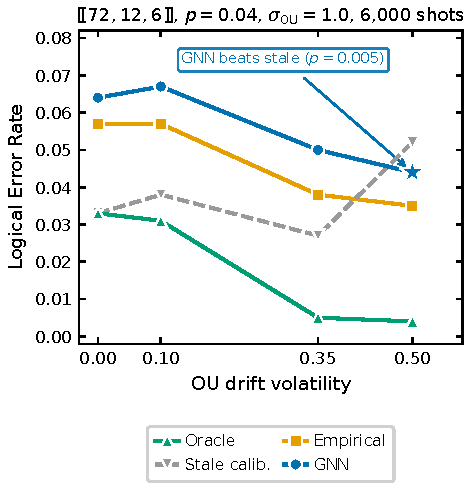
\includegraphics[width=\columnwidth]{fig_F3_drift_adaptation}
%DIFDELCMD < %%%
%DIFDELCMD < \caption{%
{%DIFAUXCMD
\DIFdelFL{LER vs.\ OU drift volatility for four decoder configurations
         on $\code{72}{12}{6}$, $p=0.04$, $\sigma_\mathrm{OU}=1.0$, 6}%DIFDELCMD < {%%%
\DIFdelFL{,}%DIFDELCMD < }%%%
\DIFdelFL{000 shots.
         Star marks the single operating point (vol$=0.5$) where GNN
         beats stale calibration ($p=0.005$); GNN is beaten by the
         empirical frequency estimator at every volatility level.}}
%DIFAUXCMD
%DIFDELCMD < \label{fig:drift_curve}
%DIFDELCMD < \end{figure}
%DIFDELCMD < %%%
\DIFdelend \DIFaddbegin \DIFadd{$p_Y=0$,
$\eta=20$, applied to every qubit after each one- and two-qubit gate and to
every idle qubit at each time step; measurements and resets flip with
probability $p$. Under spatially non-uniform noise each qubit $q$ (data and
ancilla) has rate $p_q=p_\mathrm{mean}e^{\sigma z_q}$, $z_q\sim\mathcal N(0,1)$,
$\sigma=1$, on all of its fault locations.
}\DIFaddend 

\DIFdelbegin \DIFdel{Table~\ref{tab:drift} and Fig. ~\ref{fig:drift_curve} show that the
GNN beats stale calibration
at vol$=0.5$ ($p=0.005$}\DIFdelend \DIFaddbegin \paragraph{\DIFadd{Decoders.}}
\DIFadd{We decode the detector error model (DEM; 4}{\DIFaddend ,\DIFdelbegin \DIFdel{158 vs. \ 111 discordant pairs) , but
is beaten by the non-learned empirical frequency estimator at every volatility level (GNN vs.\ empir: $p = 2.7\times10^{-8}$
at vol$=0.5$, GNN worse) . Under independent per-qubit drift,
direct per-qubit syndrome frequency counting captures most of
the available signal, leaving little room for a learned estimator.
Whether spatial correlation structure between qubits would shift
this result is an open question}\DIFdelend \DIFaddbegin }\DIFadd{068 fault mechanisms) with
BP-OSD (min-sum, scaling $0.625$, serial schedule, 100 iterations, OSD-CS
order 10). The }\emph{\DIFadd{mean-prior}} \DIFadd{decoder uses a uniform rate equal to the
log-normal mean $p_\mathrm{mean}e^{\sigma^2/2}$; the }\emph{\DIFadd{oracle}} \DIFadd{uses the
true $p_q$. We draw 20 (40) rate profiles at $p_\mathrm{mean}\le0.003$
($0.006$) and 500 shots per profile. A shot fails if the decoded fault set
does not reproduce the detection events or predicts the wrong observable flips}\DIFaddend .

\DIFdelbegin \subsection{\DIFdel{Circuit-level evaluation}}%DIFAUXCMD
\addtocounter{subsection}{-1}%DIFAUXCMD
%DIFDELCMD < \label{sec:circuit}
%DIFDELCMD < 

%DIFDELCMD < %%%
\DIFdel{\pending{Specify the complete circuit-level noise model: syndrome
extraction circuit, number of data/check qubits, gate/reset/measurement
error channels and rates, treatment of bias/Y errors, detector
construction, and BP-OSD configuration. Without these details the
circuit-level result is not reproducible.}
}%DIFDELCMD < 

%DIFDELCMD < %%%
\DIFdelend \begin{table}[t]
\centering
\caption{Circuit-level oracle gap on $\code{72}{12}{6}$ \DIFdelbeginFL \DIFdelFL{, }\DIFdelendFL \DIFaddbeginFL \DIFaddFL{(}\DIFaddendFL 6 rounds, $\eta=20$,
\DIFdelbeginFL \DIFdelFL{5}%DIFDELCMD < {%%%
\DIFdelFL{,}%DIFDELCMD < }%%%
\DIFdelFL{000 }\DIFdelendFL \DIFaddbeginFL \DIFaddFL{log-normal $\sigma=1$). $n_{10}$: }\DIFaddendFL shots \DIFdelbeginFL \DIFdelFL{per point (preliminary,
         $N=5{,}000$ }\DIFdelendFL \DIFaddbeginFL \DIFaddFL{only the mean-prior decoder fails;
$n_{01}$: }\DIFaddendFL shots \DIFdelbeginFL \DIFdelFL{, underpowered)}\DIFdelendFL \DIFaddbeginFL \DIFaddFL{only the oracle fails. The last column counts rate profiles
on which the mean-prior decoder has more failures than the oracle / fewer}\DIFaddendFL .}
\label{tab:circuit}
\DIFdelbeginFL %DIFDELCMD < \resizebox{\columnwidth}{!}{%
%DIFDELCMD < \begin{tabular}{@{}lcccc@{}}
%DIFDELCMD < \toprule
%DIFDELCMD < $p_\mathrm{mean}$ & Mean LER & Oracle LER & Discordant & McNemar $p$ \\
%DIFDELCMD < \midrule
%DIFDELCMD < 0.001 & 0.272 & 0.270 & 3 & 0.25 \\
%DIFDELCMD < 0.003 & 0.335 & 0.335 & 8 & 1.00 \\
%DIFDELCMD < \bottomrule
%DIFDELCMD < \end{tabular}}
%DIFDELCMD < %%%
\DIFdelendFL \DIFaddbeginFL \resizebox{\columnwidth}{!}{%
\begin{tabular}{@{}lccccc@{}}
\toprule
$p_\mathrm{mean}$ & Shots & Mean-prior LER & Oracle LER & $n_{10}/n_{01}$ (McNemar $p$) & Profiles \\
\midrule
0.001 & 10{,}000 & $0$ ($<\!3.8\times10^{-4}$) & $0$ ($<\!3.8\times10^{-4}$) & 0/0 & 0/0 \\
0.003 & 10{,}000 & $1.4\times10^{-3}$ & $0.6\times10^{-3}$ & 9/1 (0.027) & 6/0 \\
0.006 & 20{,}000 & $1.36\times10^{-2}$ & $0.60\times10^{-2}$ & 192/39 ($1.5\times10^{-23}$) & 38/2 \\
\bottomrule
\end{tabular}}
\DIFaddendFL \end{table}

\begin{figure}[t]
\centering
\DIFdelbeginFL %DIFDELCMD < \includegraphics[width=\columnwidth]{fig_F6_circuit_null}
%DIFDELCMD < %%%
\DIFdelendFL \DIFaddbeginFL 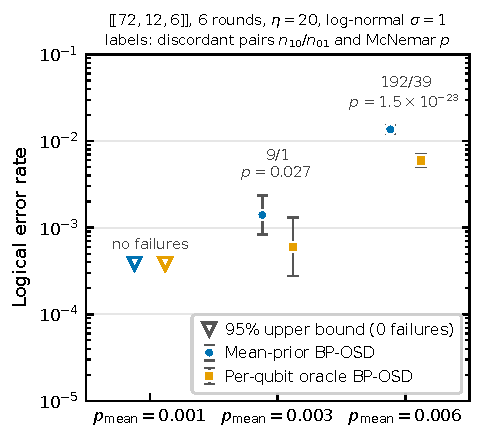
\includegraphics[width=\columnwidth]{fig_F6_circuit_oracle}
\DIFaddendFL \caption{Circuit-level oracle gap on $\code{72}{12}{6}$\DIFdelbeginFL \DIFdelFL{, 6 rounds,
         $\eta=20$, 5}%DIFDELCMD < {%%%
\DIFdelFL{,}%DIFDELCMD < }%%%
\DIFdelFL{000 shots}\DIFdelendFL . \DIFdelbeginFL \DIFdelFL{No statistically detectable
         difference between }\DIFdelendFL \DIFaddbeginFL \DIFaddFL{Points: logical
error rate with 95\% Wilson intervals; open triangles: 95\% upper bound when
no failures were observed. The per-qubit oracle has $56\%$ fewer failures
than the }\DIFaddendFL mean-prior \DIFdelbeginFL \DIFdelFL{and per-qubit-oracle BP-OSD
         }\DIFdelendFL \DIFaddbeginFL \DIFaddFL{decoder }\DIFaddendFL at \DIFdelbeginFL \DIFdelFL{either operating point (McNemar $p \geq 0.25$; 3 and 8
         discordant pairs---underpowered, see text)}\DIFdelendFL \DIFaddbeginFL \DIFaddFL{$p_\mathrm{mean}=0.006$}\DIFaddendFL .}
\DIFdelbeginFL %DIFDELCMD < \label{fig:circuit_null}
%DIFDELCMD < %%%
\DIFdelendFL \DIFaddbeginFL \label{fig:circuit_oracle}
\DIFaddendFL \end{figure}

\DIFaddbegin \DIFadd{Knowing the per-qubit rates also helps at circuit level
(}\DIFaddend Table~\ref{tab:circuit}\DIFdelbegin \DIFdel{and }\DIFdelend \DIFaddbegin \DIFadd{, }\DIFaddend Fig.~\DIFdelbegin \DIFdel{\ref{fig:circuit_null} show no
statistically detectable oracle gap at circuit level. With only 3
and 8 discordant pairs at the two tested operating points, however,
McNemar 's test cannot distinguish a true zero gap from a gap of up
to approximately $1.5\%$ LER---consistent with the }\DIFdelend \DIFaddbegin \DIFadd{\ref{fig:circuit_oracle}). At
$p_\mathrm{mean}=0.006$ the oracle reduces the logical error rate from
$1.36\%$ to $0.60\%$ ($56\%$; McNemar $p=1.5\times10^{-23}$), and it is
better on 38 of 40 independent rate profiles (sign test $p=1.5\times10^{-9}$),
so the result is not driven by a few extreme profiles. At
$p_\mathrm{mean}=0.003$ the gap has the same size ($57\%$) but only 10
discordant shots, and at $p_\mathrm{mean}=0.001$ neither decoder fails in
$10^4$ shots. The circuit-level gap ($56\%$) is somewhat smaller than the
}\DIFaddend code-capacity \DIFdelbegin \DIFdel{oracle gap }\DIFdelend \DIFaddbegin \DIFadd{gap on the same code ($65.1\%$), but it does not vanish.
}

\paragraph{\DIFadd{Correction to an earlier version.}}
\DIFadd{An earlier version of this section reported logical error rates of $0.27$ and
$0.34$ }\DIFaddend at \DIFdelbegin \DIFdel{low contrast. The present sample cannot distinguish between negligible prior
sensitivity and a nonzero gap below the
resolution of the experiment. Higher shot counts (targeting $\geq 100$ discordant
pairs)are required to distinguish these cases.
The two prior assignments are nevertheless numerically distinct: 86\%
of fault mechanisms change rank by more than 50 positions and
the
per-mechanism probability ratios span $0.25\times$--$5.1\times$. The
DEM contains 3}%DIFDELCMD < {%%%
\DIFdelend \DIFaddbegin \DIFadd{$p_\mathrm{mean}=0.001$ and $0.003$ and no oracle gap. Those
circuits lacked the first-round and final detectors (360 instead of 432),
so any fault that flipped a logical near the time boundaries was invisible
to the decoder. This produced a logical error floor that no prior could
remove. With the complete detector set, uniform noise at $p=0.001$}\DIFaddend , \DIFdelbegin %DIFDELCMD < }%%%
\DIFdel{821 fault mechanisms and 360 detectors }\DIFdelend \DIFaddbegin \DIFadd{$0.003$}\DIFaddend ,
\DIFdelbegin \DIFdel{suggesting that
many fault mechanisms map to the same detector information. This high degeneracy is a plausible explanation for the weak prior
sensitivity, but the present experiment does not isolate it causally.
An ablation that changes DEM degeneracy while holding the prior mismatch
fixed would be required for that conclusion. }%DIFDELCMD < 

%DIFDELCMD < %%%
\DIFdel{Thus, the circuit-level experiment is currently a null result with
insufficient statistical resolution; it does not establish that
calibration side information is irrelevant at circuit level}\DIFdelend \DIFaddbegin \DIFadd{$0.005$ and $0.01$ gives $0/10^4$, $5/10^4$, $14/10^4$ and
$2.1\times10^{-2}$; the legacy circuit gives $0.124$ and $0.336$ at
$p=0.001$ and $0.003$}\DIFaddend .

% ============================================================
%  VI. DISCUSSION
% ============================================================
\section{Discussion}\label{sec:discussion}

\subsection{The GNN's role and its limits}

\textsc{TannerGNN} \DIFdelbegin \DIFdel{achieves a $15.4\%$ LER reduction over the }\DIFdelend \DIFaddbegin \DIFadd{reduces the LER of the 10-iteration }\DIFaddend flooding BP
decoder used in its training loop \DIFdelbegin \DIFdel{. The paired held-out test supports a real difference for this trained checkpoint, while gradient diagnostics
show that the network produces non-trivial corrections. Robustness to
training initialization has not yet been measured, so we do not treat the single-seed result as a reproducibility claim}\DIFdelend \DIFaddbegin \DIFadd{by $12.5\%\pm0.6\%$ over five training
seeds, and the gain persists outside the training range. The mechanism is
mainly convergence: the GNN roughly halves the number of shots on which BP
fails to reach a syndrome-consistent estimate (1}{\DIFadd{,}}\DIFadd{740 to 838--975 of
20}{\DIFadd{,}}\DIFadd{000). Running BP for 100 iterations achieves more than this, and
BP-OSD more still, so the result is best read as a cheaper route to part
of the benefit of longer decoding, not as an improvement on
state-of-the-art BB decoding}\DIFaddend .

The Regime-B result \DIFdelbegin \DIFdel{is also informative: the learned correction does
not transfer automatically to serial }\DIFdelend \DIFaddbegin \DIFadd{follows from the failure-set structure
(Table~\ref{tab:failure_sets}): }\DIFaddend BP-OSD\DIFdelbegin \DIFdel{. This is consistent with the
training/evaluation mismatch, but the residual failure sets have not yet
been characterized well enough to claim a trapping-set mechanism}\DIFdelend \DIFaddbegin \DIFadd{'s failures are a near-subset of
BP's, and the GNN's repairs fall mostly on shots BP-OSD already decodes.
When passed to BP-OSD, the learned corrections reshuffle failures among
the hardest shots and make OSD choose heavier incorrect estimates, giving
a small net loss}\DIFaddend . Training against \DIFdelbegin \DIFdel{BP-OSD directly is complicated by the non-differentiable
OSD stage; differentiable surrogates, distillation, or training }\DIFdelend \DIFaddbegin \DIFadd{the target decoder, for example
through a differentiable surrogate of OSD or }\DIFaddend on the residual failures of
\DIFdelbegin \DIFdel{the target decoder are possible alternatives}\DIFdelend \DIFaddbegin \DIFadd{BP-OSD, is the appropriate next test}\DIFaddend .

\subsection{Benchmark design implications}

The baseline experiments identify two reporting requirements for learned
QLDPC decoders. First, BP-OSD schedule, update rule, iteration count, and
OSD configuration must be stated explicitly because they can change LER
by more than two orders of magnitude on the same code. Table~\ref{tab:hparams}
records these settings for the present study.

Second, the training and evaluation decoders must be distinguished. An
LLR correction learned through flooding BP need not remain beneficial
when the schedule, iteration count, and OSD stage are changed. Comparisons
across such decoder configurations should identify the mismatch rather
than treating all BP-based baselines as equivalent.

\subsection{Comparison with prior work}\label{sec:priorwork}

Astra~\cite{Maan2025MLBP} uses a learned Tanner-graph message-passing
decoder and reports BB-code performance competitive with, and in several
settings better than, BP-OSD under code-capacity depolarizing noise. This
places our \DIFdelbegin \DIFdel{$15.4\%$ }\DIFdelend \DIFaddbegin \DIFadd{$12.5\%$ }\DIFaddend flooding-BP gain in context: improvement over plain BP
is not, by itself, the main novelty. Our contribution is instead the
controlled comparison showing how that gain changes when the baseline
and side information are strengthened.

Gong et al.~\cite{Gong2024GNN} interleave differentiable BP stages with
GNN corrections on the same sparse graph and show error-floor
improvements over several post-processing approaches. Our interleaved
variant follows the same broad design principle, but \DIFdelbegin \DIFdel{the checkpoint
reported here does not train successfully. We therefore do not claim a
competitive result }\DIFdelend \DIFaddbegin \DIFadd{its decoding
performance is not evaluated here, so we make no claim }\DIFaddend for that
architecture.

Recent circuit-level work on BB codes also reports neural decoders that
can outperform BP-OSD on the $\code{72}{12}{6}$ code while retaining a
runtime advantage, although scaling to $\code{144}{12}{12}$ remains more
challenging~\cite{Blue2026MLBB}. This comparison reinforces the need to evaluate learned decoders against
a fully specified competitive non-learned baseline, not only against
flooding BP.

Stein et al.~\cite{Stein2026FiLM} condition a neural QEC decoder on
spatially resolved hardware calibration data using FiLM and evaluate on
IBM repetition-code experiments. Their conditioning signal is per-qubit
and calibration-derived, unlike the single scalar $\phat$ used in our
initial model. This distinction is consistent with the oracle experiments
of Sec.~\ref{sec:oraclegap}, which motivate spatial rather than purely
global conditioning.
\subsection{Towards spatially-resolved conditioning}\label{sec:srcf}

The oracle-gap experiment (Sec.~\ref{sec:oraclegap}) shows that
per-qubit rate side information can materially improve the tested
BP-OSD decoder. Because operating point and code size co-vary, the
current data do not establish how this value scales with distance.
Proposition~\ref{prop:invariance} also shows that a uniform rescaling
of the min-sum BP prior cannot reproduce the effect of spatially varying
reliabilities. These results motivate testing spatially resolved FiLM
(SRCF), in which per-qubit parameters $(\gamma_i, \beta_i)$ are
conditioned on persistent hardware calibration data rather than on a
single graph-wide scalar. Such a decoder should be compared with \DIFdelbegin \DIFdel{the
}\DIFdelend \DIFaddbegin \DIFadd{a }\DIFaddend non-learned \DIFdelbegin \DIFdel{frequency estimator of Sec.~\ref{sec:drift} and evaluated in a circuit-level setting where the calibration signal remains
identifiable.Neither condition has
}\DIFdelend \DIFaddbegin \DIFadd{per-qubit frequency
estimator and evaluated at circuit level, where the oracle gap remains
large ($56\%$ at $p_\mathrm{mean}=0.006$, Sec.~\ref{sec:circuit}).
Whether such rates can be estimated well enough from syndrome history has
not }\DIFaddend been established in the present experiments.

\subsection{Limitations}\label{sec:limitations}

\DIFdelbegin %DIFDELCMD < \begin{enumerate}[leftmargin=*,topsep=3pt,itemsep=2pt,
%DIFDELCMD <                   label=(\roman*)]
%DIFDELCMD < %%%
\DIFdelend \DIFaddbegin \begin{enumerate}[leftmargin=*,topsep=3pt,itemsep=2pt,label=(\roman*)]
\DIFaddend \item The \DIFdelbegin \DIFdel{primary $15.4\%$ GNN result uses one training seed. Statistical
      uncertainty over independent training runs has not been measured.
}%DIFDELCMD < \item %%%
\item%DIFAUXCMD
\DIFdel{All GNN variants were trained against }\DIFdelend \DIFaddbegin \DIFadd{GNN was trained only through }\DIFaddend 10-iteration flooding BP. \DIFdelbegin \DIFdel{No variant was trained }\DIFdelend \DIFaddbegin \DIFadd{Training
      }\DIFaddend against serial BP-OSD, \DIFdelbegin \DIFdel{which is }\DIFdelend the competitive classical baseline\DIFdelbegin \DIFdel{. Whether GNN
      augmentation of serial BP-OSD yields gains }\DIFdelend \DIFaddbegin \DIFadd{, }\DIFaddend is untested.
\item GNN checkpoints exist only for $\code{72}{12}{6}$; the larger codes
      were not trained \DIFdelbegin \DIFdel{due to }\DIFdelend \DIFaddbegin \DIFadd{because of }\DIFaddend CPU-only compute\DIFdelbegin \DIFdel{constraints. The null result
      in Regime B }\DIFdelend \DIFaddbegin \DIFadd{. The Regime-B result
      }\DIFaddend should not be extrapolated to \DIFdelbegin \DIFdel{the larger codes.
}%DIFDELCMD < \item %%%
\item%DIFAUXCMD
\DIFdel{The interleaved model reached its best validation checkpoint at epoch 1,
      after which the validation loss increased. The current run is therefore
      insufficient to evaluate the interleaved architecture.
}%DIFDELCMD < \item %%%
\item%DIFAUXCMD
\DIFdel{All training and evaluation used CPU only, which limited
      hyperparameter search and training duration}\DIFdelend \DIFaddbegin \DIFadd{them}\DIFaddend .
\item The single per-qubit correction \DIFdelbegin \DIFdel{$\Delta_i$ is }\DIFdelend \DIFaddbegin \DIFadd{$\delta_j$ is trained on $Z$ errors
      and }\DIFaddend applied to both \DIFdelbegin \DIFdel{$\llr_{z,i}$ and $\llr_{x,i}$}\DIFdelend \DIFaddbegin \DIFadd{CSS components}\DIFaddend , which is suboptimal under
      \DIFdelbegin \DIFdel{$\eta = 20$ }\DIFdelend \DIFaddbegin \DIFadd{$\eta=20$ }\DIFaddend biased noise; separate $Z$ \DIFdelbegin \DIFdel{/}\DIFdelend \DIFaddbegin \DIFadd{and }\DIFaddend $X$ readout heads are the
      \DIFdelbegin \DIFdel{recommended }\DIFdelend \DIFaddbegin \DIFadd{natural }\DIFaddend fix.
\item \DIFdelbegin \DIFdel{Code-capacity noise omits measurement errors, leakage, and correlated faults present in real circuits}\DIFdelend \DIFaddbegin \DIFadd{The interleaved architecture and the FiLM variant are described but
      their decoding performance is not evaluated.
}\item \DIFadd{The circuit-level study uses one code, 6 rounds and a biased
      single-qubit channel after each gate; two-qubit correlated faults,
      leakage and crosstalk are not modelled, and the paper's operating
      points $p_\mathrm{mean}\le0.003$ are too clean to resolve the gap.
}\item \DIFadd{Hyperparameter search and training duration were limited by CPU-only
      compute}\DIFaddend .
\end{enumerate}

% ============================================================
%  VII. CONCLUSION
% ============================================================
\section{Conclusion}\label{sec:conclusion}

On $\code{72}{12}{6}$, a Tanner-graph GNN trained through 10-iteration
flooding BP reduces \DIFdelbegin \DIFdel{the held-out LER by $15.4\%$ }\DIFdelend \DIFaddbegin \DIFadd{that decoder's LER by $12.5\%\pm0.6\%$ }\DIFaddend at $p=0.04$
and \DIFdelbegin \DIFdel{$\eta=20$. The same learned correction does not improve the
serial min-sum }\DIFdelend \DIFaddbegin \DIFadd{$10.6\%\pm0.7\%$ at $p=0.06$, reproducibly over five training seeds
and on leakage-free held-out data. The gain comes mostly from helping BP
converge. It does not reach 100-iteration BP or serial }\DIFaddend BP-OSD\DIFdelbegin \DIFdel{reference decoder and increases LER at the
two
highest tested error rates. The demonstrated gain is therefore specific
to the training-aligned flooding-BP baseline ; the present experiments do
}\DIFdelend \DIFaddbegin \DIFadd{, and the
same corrections make BP-OSD slightly worse because the shots they repair
are largely ones BP-OSD already decodes. An improvement over one BP
baseline therefore does }\DIFaddend not establish an improvement over \DIFdelbegin \DIFdel{competitive BB decoding more generally}\DIFdelend \DIFaddbegin \DIFadd{a stronger
decoder}\DIFaddend .

\DIFdelbegin \DIFdel{The baseline experiments show that BP schedule, update rule, iteration
budget, and OSD configuration can change finite-length LER by
orders of
magnitude. These parameters must be treated as part of the decoder
specification when learned and non-learned methods are compared. We also
}\DIFdelend \DIFaddbegin \DIFadd{Decoder configuration matters as much as the learned component: on
$\code{288}{12}{18}$, schedule and OSD post-processing alone change LER by
about $47\times$. We }\DIFaddend proved that uniform positive rescaling of the channel
LLRs leaves the hard decisions of \DIFdelbegin \DIFdel{ideal }\DIFdelend \DIFaddbegin \DIFadd{unclipped }\DIFaddend min-sum BP unchanged\DIFdelbegin \DIFdel{. A global prior magnitude
alone therefore cannot provide spatial adaptation to heterogeneous qubit
reliabilities, although a nonlinear learned model may still use }\DIFdelend \DIFaddbegin \DIFadd{, so }\DIFaddend a
global noise estimate \DIFdelbegin \DIFdel{as context. }%DIFDELCMD < 

%DIFDELCMD < %%%
\DIFdel{The synthetic oracle experiments identify per-qubit calibrationas the
more informative adaptive signal in the tested setting: revealing the
}\DIFdelend \DIFaddbegin \DIFadd{cannot by itself make min-sum BP adaptive. Per-qubit
calibration, in contrast, is highly informative: revealing }\DIFaddend true per-qubit
rates \DIFdelbegin \DIFdel{substantially improves }\DIFdelend \DIFaddbegin \DIFadd{reduces }\DIFaddend BP-OSD\DIFdelbegin \DIFdel{under heterogeneous
}\DIFdelend \DIFaddbegin \DIFadd{'s LER by up to $88\%$ at code capacity and by $56\%$
under circuit-level }\DIFaddend noise. The \DIFdelbegin \DIFdel{current cross-code experiments do not isolate how this gain
scales with distance, and the circuit-level study does not yet have
sufficient statistical resolution. A }\DIFdelend direct next test is \DIFdelbegin \DIFdel{to condition }\DIFdelend a learned decoder
\DIFaddbegin \DIFadd{conditioned }\DIFaddend on persistent spatial calibration data\DIFdelbegin \DIFdel{and compare it
}\DIFdelend \DIFaddbegin \DIFadd{, compared }\DIFaddend against a
fully specified serial BP-OSD baseline and \DIFdelbegin \DIFdel{the }\DIFdelend \DIFaddbegin \DIFadd{a }\DIFaddend non-learned \DIFdelbegin \DIFdel{frequency estimator, using multiple training seeds and a noise model that
preserves temporal calibration structure.
}\DIFdelend \DIFaddbegin \DIFadd{per-qubit
estimator.
}

\DIFaddend \section*{Acknowledgments}

The authors thank the STAR Lab program at the University of Arizona
for facilitating this research and providing computational resources.

\section*{Data and code availability}

Source code, trained checkpoints, \DIFdelbegin \DIFdel{all datasets , and the audit scripts that produced the findings of Secs.~\ref{sec:baseline}
and~\ref{sec:invariance} }\DIFdelend \DIFaddbegin \DIFadd{datasets and analysis scripts }\DIFaddend are
available at \DIFdelbegin %DIFDELCMD < \url{https://github.com/anish-chedalla/adaptive_gnn}%%%
\DIFdel{.
Syndrome data were generated using }\DIFdelend \DIFaddbegin \url{https://github.com/kondshk/adaptive_gnn}\DIFadd{.
All tables and figures are produced by a committed script from stored
per-shot outcomes: }\texttt{\DIFadd{audit\_headline\_v2.py}} \DIFadd{(headline result),
}\texttt{\DIFadd{audit\_tables\_v2.py}} \DIFadd{(baseline, invariance, BP-OSD and oracle
tables), }\texttt{\DIFadd{audit\_failure\_sets.py}} \DIFadd{(failure sets) and
}\texttt{\DIFadd{audit\_circuit\_v2.py}} \DIFadd{(circuit level); }\texttt{\DIFadd{docs/PROVENANCE.md}}
\DIFadd{maps each reported number to its source. Code-capacity data are sampled directly with NumPy;
circuit-level data are generated with }\DIFaddend Stim~\cite{Gidney2021Stim}.

\bibliographystyle{quantum}
\bibliography{references}

\end{document}
